% Options for packages loaded elsewhere
\PassOptionsToPackage{unicode}{hyperref}
\PassOptionsToPackage{hyphens}{url}
%
\documentclass[
]{book}
\usepackage{amsmath,amssymb}
\usepackage{iftex}
\ifPDFTeX
  \usepackage[T1]{fontenc}
  \usepackage[utf8]{inputenc}
  \usepackage{textcomp} % provide euro and other symbols
\else % if luatex or xetex
  \usepackage{unicode-math} % this also loads fontspec
  \defaultfontfeatures{Scale=MatchLowercase}
  \defaultfontfeatures[\rmfamily]{Ligatures=TeX,Scale=1}
\fi
\usepackage{lmodern}
\ifPDFTeX\else
  % xetex/luatex font selection
\fi
% Use upquote if available, for straight quotes in verbatim environments
\IfFileExists{upquote.sty}{\usepackage{upquote}}{}
\IfFileExists{microtype.sty}{% use microtype if available
  \usepackage[]{microtype}
  \UseMicrotypeSet[protrusion]{basicmath} % disable protrusion for tt fonts
}{}
\makeatletter
\@ifundefined{KOMAClassName}{% if non-KOMA class
  \IfFileExists{parskip.sty}{%
    \usepackage{parskip}
  }{% else
    \setlength{\parindent}{0pt}
    \setlength{\parskip}{6pt plus 2pt minus 1pt}}
}{% if KOMA class
  \KOMAoptions{parskip=half}}
\makeatother
\usepackage{xcolor}
\usepackage{color}
\usepackage{fancyvrb}
\newcommand{\VerbBar}{|}
\newcommand{\VERB}{\Verb[commandchars=\\\{\}]}
\DefineVerbatimEnvironment{Highlighting}{Verbatim}{commandchars=\\\{\}}
% Add ',fontsize=\small' for more characters per line
\usepackage{framed}
\definecolor{shadecolor}{RGB}{248,248,248}
\newenvironment{Shaded}{\begin{snugshade}}{\end{snugshade}}
\newcommand{\AlertTok}[1]{\textcolor[rgb]{0.94,0.16,0.16}{#1}}
\newcommand{\AnnotationTok}[1]{\textcolor[rgb]{0.56,0.35,0.01}{\textbf{\textit{#1}}}}
\newcommand{\AttributeTok}[1]{\textcolor[rgb]{0.13,0.29,0.53}{#1}}
\newcommand{\BaseNTok}[1]{\textcolor[rgb]{0.00,0.00,0.81}{#1}}
\newcommand{\BuiltInTok}[1]{#1}
\newcommand{\CharTok}[1]{\textcolor[rgb]{0.31,0.60,0.02}{#1}}
\newcommand{\CommentTok}[1]{\textcolor[rgb]{0.56,0.35,0.01}{\textit{#1}}}
\newcommand{\CommentVarTok}[1]{\textcolor[rgb]{0.56,0.35,0.01}{\textbf{\textit{#1}}}}
\newcommand{\ConstantTok}[1]{\textcolor[rgb]{0.56,0.35,0.01}{#1}}
\newcommand{\ControlFlowTok}[1]{\textcolor[rgb]{0.13,0.29,0.53}{\textbf{#1}}}
\newcommand{\DataTypeTok}[1]{\textcolor[rgb]{0.13,0.29,0.53}{#1}}
\newcommand{\DecValTok}[1]{\textcolor[rgb]{0.00,0.00,0.81}{#1}}
\newcommand{\DocumentationTok}[1]{\textcolor[rgb]{0.56,0.35,0.01}{\textbf{\textit{#1}}}}
\newcommand{\ErrorTok}[1]{\textcolor[rgb]{0.64,0.00,0.00}{\textbf{#1}}}
\newcommand{\ExtensionTok}[1]{#1}
\newcommand{\FloatTok}[1]{\textcolor[rgb]{0.00,0.00,0.81}{#1}}
\newcommand{\FunctionTok}[1]{\textcolor[rgb]{0.13,0.29,0.53}{\textbf{#1}}}
\newcommand{\ImportTok}[1]{#1}
\newcommand{\InformationTok}[1]{\textcolor[rgb]{0.56,0.35,0.01}{\textbf{\textit{#1}}}}
\newcommand{\KeywordTok}[1]{\textcolor[rgb]{0.13,0.29,0.53}{\textbf{#1}}}
\newcommand{\NormalTok}[1]{#1}
\newcommand{\OperatorTok}[1]{\textcolor[rgb]{0.81,0.36,0.00}{\textbf{#1}}}
\newcommand{\OtherTok}[1]{\textcolor[rgb]{0.56,0.35,0.01}{#1}}
\newcommand{\PreprocessorTok}[1]{\textcolor[rgb]{0.56,0.35,0.01}{\textit{#1}}}
\newcommand{\RegionMarkerTok}[1]{#1}
\newcommand{\SpecialCharTok}[1]{\textcolor[rgb]{0.81,0.36,0.00}{\textbf{#1}}}
\newcommand{\SpecialStringTok}[1]{\textcolor[rgb]{0.31,0.60,0.02}{#1}}
\newcommand{\StringTok}[1]{\textcolor[rgb]{0.31,0.60,0.02}{#1}}
\newcommand{\VariableTok}[1]{\textcolor[rgb]{0.00,0.00,0.00}{#1}}
\newcommand{\VerbatimStringTok}[1]{\textcolor[rgb]{0.31,0.60,0.02}{#1}}
\newcommand{\WarningTok}[1]{\textcolor[rgb]{0.56,0.35,0.01}{\textbf{\textit{#1}}}}
\usepackage{longtable,booktabs,array}
\usepackage{calc} % for calculating minipage widths
% Correct order of tables after \paragraph or \subparagraph
\usepackage{etoolbox}
\makeatletter
\patchcmd\longtable{\par}{\if@noskipsec\mbox{}\fi\par}{}{}
\makeatother
% Allow footnotes in longtable head/foot
\IfFileExists{footnotehyper.sty}{\usepackage{footnotehyper}}{\usepackage{footnote}}
\makesavenoteenv{longtable}
\usepackage{graphicx}
\makeatletter
\def\maxwidth{\ifdim\Gin@nat@width>\linewidth\linewidth\else\Gin@nat@width\fi}
\def\maxheight{\ifdim\Gin@nat@height>\textheight\textheight\else\Gin@nat@height\fi}
\makeatother
% Scale images if necessary, so that they will not overflow the page
% margins by default, and it is still possible to overwrite the defaults
% using explicit options in \includegraphics[width, height, ...]{}
\setkeys{Gin}{width=\maxwidth,height=\maxheight,keepaspectratio}
% Set default figure placement to htbp
\makeatletter
\def\fps@figure{htbp}
\makeatother
\setlength{\emergencystretch}{3em} % prevent overfull lines
\providecommand{\tightlist}{%
  \setlength{\itemsep}{0pt}\setlength{\parskip}{0pt}}
\setcounter{secnumdepth}{5}
\usepackage{booktabs}
\usepackage{lscape}

\ifLuaTeX
  \usepackage{selnolig}  % disable illegal ligatures
\fi
\usepackage[]{natbib}
\bibliographystyle{apalike}
\IfFileExists{bookmark.sty}{\usepackage{bookmark}}{\usepackage{hyperref}}
\IfFileExists{xurl.sty}{\usepackage{xurl}}{} % add URL line breaks if available
\urlstyle{same}
\hypersetup{
  pdftitle={Econometrics},
  pdfauthor={Bakti Siregar, M.Sc},
  hidelinks,
  pdfcreator={LaTeX via pandoc}}

\title{Econometrics}
\author{Bakti Siregar, M.Sc}
\date{2023-11-29}

\begin{document}
\maketitle

{
\setcounter{tocdepth}{1}
\tableofcontents
}
\hypertarget{foreword}{%
\chapter*{Foreword}\label{foreword}}
\addcontentsline{toc}{chapter}{Foreword}

Welcome to the exciting and complex world of econometrics! This book is designed to provide an in-depth understanding of the basic concepts and practical applications in econometric analysis. Econometrics is a branch of economics that combines economic theory with mathematical and statistical methods to test economic hypotheses and make predictions about economic phenomena in the real world.

This book was prepared with the aim of providing a comprehensive guide, starting from the basics of econometrics to advanced applications relevant to the contemporary world of economics. Readers will be guided through basic concepts such as linear regression, the assumptions underlying econometric models, to sophisticated data analysis techniques.

Emphasis is placed on the application of econometrics in the context of modern economics, with relevant case studies and applicable examples. The book also integrates the latest developments in the field of econometrics, ensuring that readers gain insight into the latest approaches and methodological developments.

As the author, I hope that this book will not only be a valuable reference source for students, academics, and economic practitioners, but will also inspire further interest and understanding of the complexity of economic phenomena. I would like to thank everyone who has contributed and supported me in the process of writing this book.

\hypertarget{summary}{%
\section*{Summary}\label{summary}}
\addcontentsline{toc}{section}{Summary}

Econometrics is a branch of economics that uses mathematical and statistical methods to analyze and test hypotheses in an economic context. It combines economic concepts with statistical tools to understand and model economic relationships.

Here are some common topics in econometrics:

\begin{itemize}
\item
  \textbf{Regression Models:} Econometrics often begins with the study of regression models, in which the relationship between one or more dependent and independent variables is explained. Regression models can be simple or complex depending on the data and problem at hand.
\item
  \textbf{Regression Assumptions:} Regression analysis requires several assumptions, such as the homoscedasticity assumption (constant residual variance), the residual independence assumption, and the residual normality assumption.
\item
  \textbf{Parameter Estimation:} Using empirical data, we can estimate parameters in a regression model to find out how well the model fits the data.
\item
  \textbf{Hypothesis Testing:} Econometrics is used to test statistical hypotheses about model parameters. This helps determine whether the observed relationship is significantly different from zero.
\item
  \textbf{Multicollinearity and Heteroscedasticity:} Some common problems in regression analysis involve multicollinearity (high correlation between independent variables) and heteroscedasticity (non-constant residual variance). Econometricians develop methods to deal with these problems.
\item
  \textbf{Time Series Model:} Econometrics is also often used to analyze time series data, which includes observations taken sequentially over a certain time.
\item
  \textbf{Applied Econometrics:} In addition to basic models, econometrics is also applied in various fields of economics, including finance, human resources, marketing, and others.
\end{itemize}

\hypertarget{writer}{%
\section*{Writer}\label{writer}}
\addcontentsline{toc}{section}{Writer}

\begin{itemize}
\tightlist
\item
  \textbf{\href{https://www.linkedin.com/in/dsciencelabs/}{Bakti Siregar, M.Sc}} is Head of the Study Program at the Department of Statistics, Matana University. Graduate of Masters in Applied Mathematics from National Sun Yat Sen University, Taiwan. He is also a lecturer and Data Scientist consultant at well-known companies such as \href{https://www.jne.co.id/id/beranda}{JNE}, \href{https://www.samoragroup.co.\%20id/home/en}{Samora Group}, \href{https://www.pertamina.com/}{Pertamina}, and others. He has special enthusiasm in teaching Big Data Analytics, Machine Learning, Optimization, and Time Series Analysis in the fields of finance and investment. His expertise is also evident in the use of Statistical programming languages such as R Studio and Python. He applies the MySQL/NoSQL database system in learning data management, and is proficient in using Big Data tools such as Spark and Hadoop. Some of his projects can be seen at the following links: \href{https://rpubs.com/dsciencelabs}{Rpubs}, \href{https://github.com/dsciencelabs}{Github}, \href{https://dsciencelabs.github\%20.io/web/index.html}{Website}, and \href{https://www.kaggle.com/baktisiregar/code}{Kaggle}.
\end{itemize}

\hypertarget{my-gratitude}{%
\section*{My Gratitude}\label{my-gratitude}}
\addcontentsline{toc}{section}{My Gratitude}

Thank you to fellow academics and econometric practitioners who have shared their knowledge and insights, provided valuable input, and provided inspiration in preparing this material. I would also like to thank my family and friends who provided moral support and encouragement during the writing process. You are a source of strength and inspiration for me. The entire process of writing this was an incredible journey, and I hope this ebook will be of benefit to readers, both those who are studying econometrics for the first time and those who want to improve their understanding.

Finally, thank you to the publishing team who has worked hard in the production process of this ebook. Hopefully this ebook will be a useful reference source and can contribute to the development of econometric studies.

\hypertarget{feedback-suggestions}{%
\section*{Feedback \& Suggestions}\label{feedback-suggestions}}
\addcontentsline{toc}{section}{Feedback \& Suggestions}

All your input and feedback means a lot to us to improve this template in the future. For readers/users who wish to submit input and responses, please use the contact below!

\textbf{Email:} \href{mailto:dsciencelabs@outlook.com}{\nolinkurl{dsciencelabs@outlook.com}}

\hypertarget{introduction-to-econometrics}{%
\chapter{Introduction to Econometrics}\label{introduction-to-econometrics}}

\hypertarget{what-is-econometrics}{%
\section{What is Econometrics?}\label{what-is-econometrics}}

Econometrics is a branch of economics that combines economic concepts, mathematics, and statistics to analyze and measure empirical relationships in the economy. The term ``econometrics'' comes from combining the words ``economics'' and ``metrics'' (which means measurement). The main goal of econometrics is to develop mathematical models that can be used to explain and predict economic behavior, as well as test economic hypotheses and policies.

\begin{center}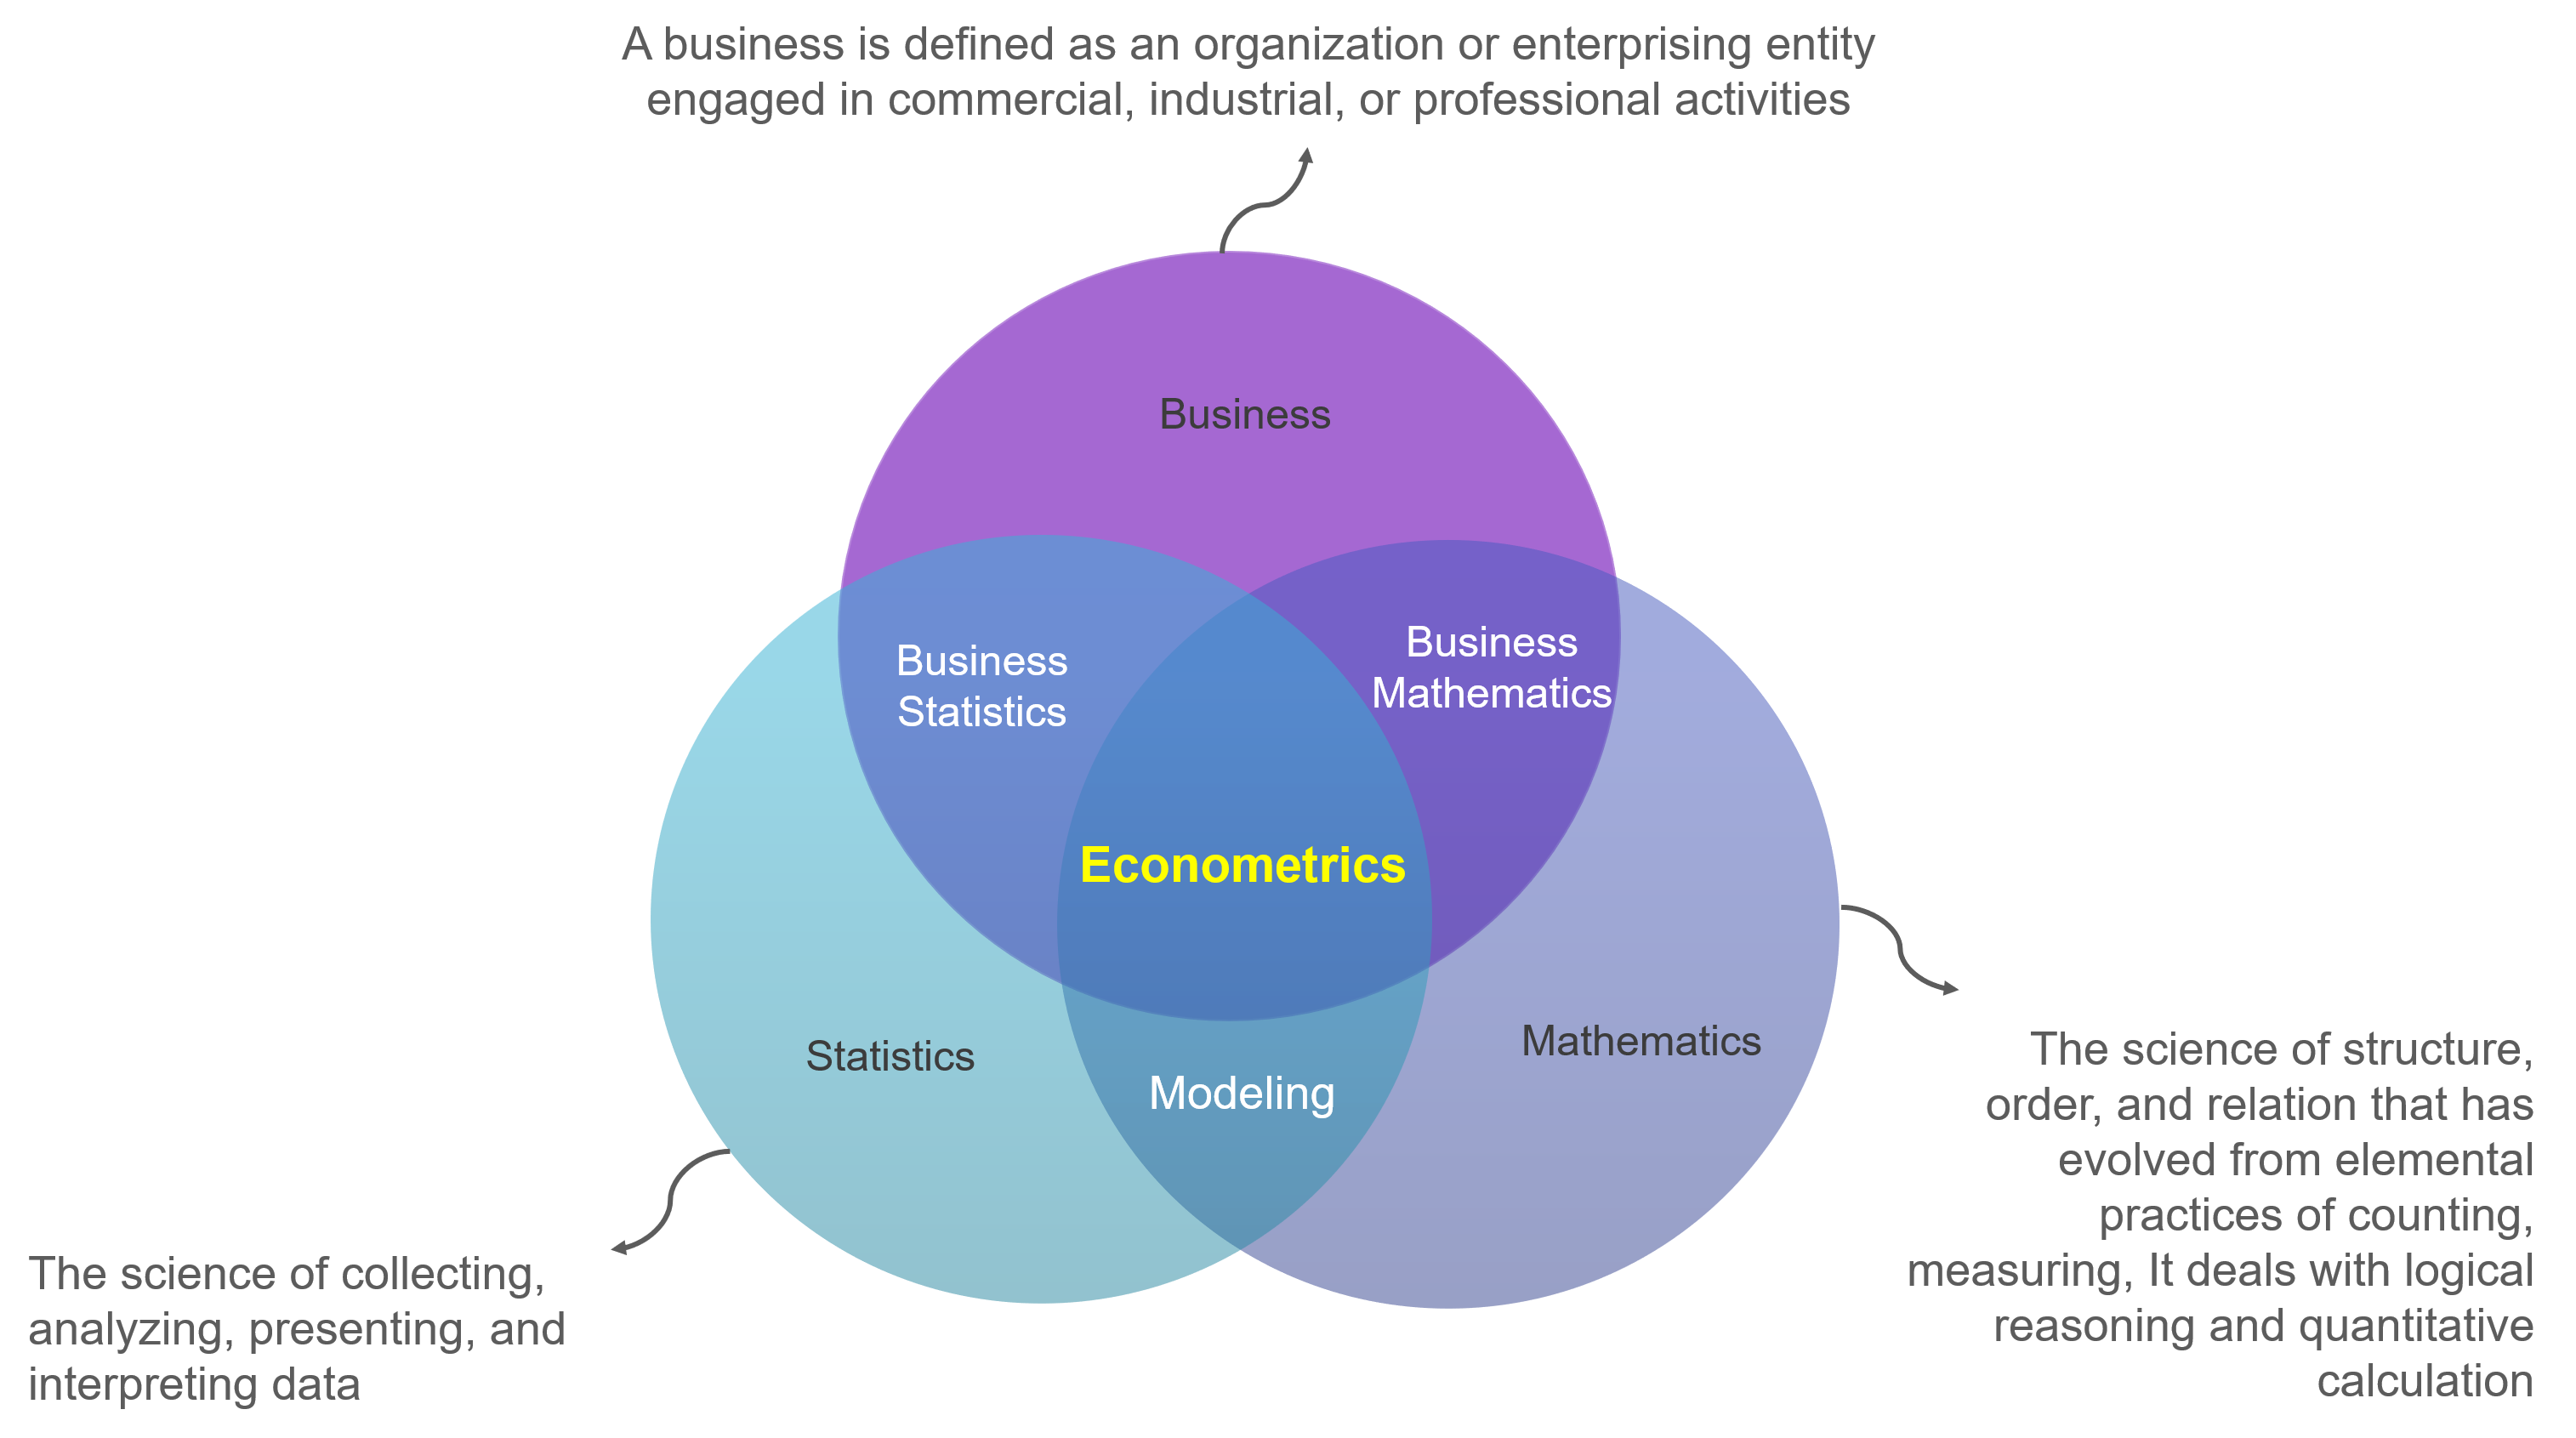
\includegraphics[width=1\linewidth]{images/Bab1/econometrics} \end{center}

In practice, econometrics involves applying statistical models to examine relationships between economic variables. By using empirical data, econometricians (econometric practitioners) try to formulate mathematical models that can explain or predict economic behavior in the real world. The main method in econometrics involves statistical regression, in which economic variables are explained and related to each other.

Some basic concepts in econometrics involve:

\begin{itemize}
\tightlist
\item
  \textbf{Regression Model:} Create a mathematical model that describes the relationship between the dependent variable and the independent variable.
\item
  \textbf{Hypothesis and Statistical Test:} Develop and test hypotheses about relationships between variables, and determine the extent to which analysis results are statistically reliable.
\item
  \textbf{Prediction:} Uses an econometric model to predict the value of the dependent variable based on the value of the given independent variable.
\item
  \textbf{Economic Policy Evaluation:} Analyze the effects of economic policies using econometric models.
\end{itemize}

Econometrics has an important role in economic and policy analysis. This allows economists to use empirical data and statistical methods to make more informational and evidence-based decisions in an economic context.

\hypertarget{goals-of-econometrics}{%
\section{Goals of Econometrics}\label{goals-of-econometrics}}

The main goal of econometrics is to develop mathematical models that can describe and explain the relationships between economic variables, as well as test economic hypotheses using empirical data. Some specific goals of econometrics involve:

\begin{itemize}
\tightlist
\item
  \textbf{Description and Measurement of Economic Relationships:} Econometrics aims to describe and measure the relationships between economic variables. This involves developing a mathematical model that reflects these relationships.
\item
  \textbf{Economic Hypothesis Testing:} Econometrics is used to test economic hypotheses, such as whether there is a causal relationship between two variables or whether the effects of an economic policy are significant.
\item
  \textbf{Forecasting and Prediction:} Econometrics provides tools for making forecasts and predictions about future economic behavior. By using the developed model, econometricians can estimate the value of the dependent variable based on the value of the given independent variable.
\item
  \textbf{Economic Policy Evaluation:} Econometrics is used to evaluate the impact of economic policies. This allows economists to understand how changes in certain economic variables can affect other variables, thereby helping in policy decision making.
\item
  \textbf{Understanding of Economic Processes:} Through statistical analysis, econometrics can help in deep understanding of complex economic processes. This includes identifying factors that influence the behavior of consumers, producers, and the market as a whole.
\item
  \textbf{Empirical Research:} Econometrics provides tools for economic researchers to test economic theories using empirical data. This can help fill the gap between economic theory and the economic reality that occurs on the ground.
\item
  \textbf{Evidence-Based Decision Making:} One of the main goals of econometrics is to provide an empirical basis for decision making in an economic context. By using data and statistical methods, econometrics helps make more informed and evidence-based decisions.
\end{itemize}

Thus, econometrics has an important role in providing powerful analytical tools for economists to understand and interpret economic phenomena in the real world.

\hypertarget{econometric-relations-and-regression}{%
\section{Econometric Relations and Regression}\label{econometric-relations-and-regression}}

Regression is a very important analytical tool in econometrics, helping researchers and analysts to measure and understand economic relationships based on empirical data.

\begin{itemize}
\tightlist
\item
  \textbf{Use of Regression in Econometrics:} Regression is one of the main tools in econometric analysis. Econometricians use regression techniques to estimate parameters and measure relationships between economic variables.
\item
  \textbf{Regression Models in Econometrics:} In the context of econometrics, regression models are often used to describe and understand causal relationships between economic variables. This model can include economic variables such as income, prices, production, and others.
\item
  \textbf{Hypothesis Testing in Regression Context:} Econometricians use regression to test economic hypotheses. For example, does an increase in variable A cause an increase or decrease in variable B.
\item
  \textbf{Prediction and Forecasting:} Regression analysis is used in econometrics to make predictions and forecasting. By using a regression model, econometricians can estimate the value of the dependent variable based on the value of the independent variable.
\end{itemize}

\begin{center}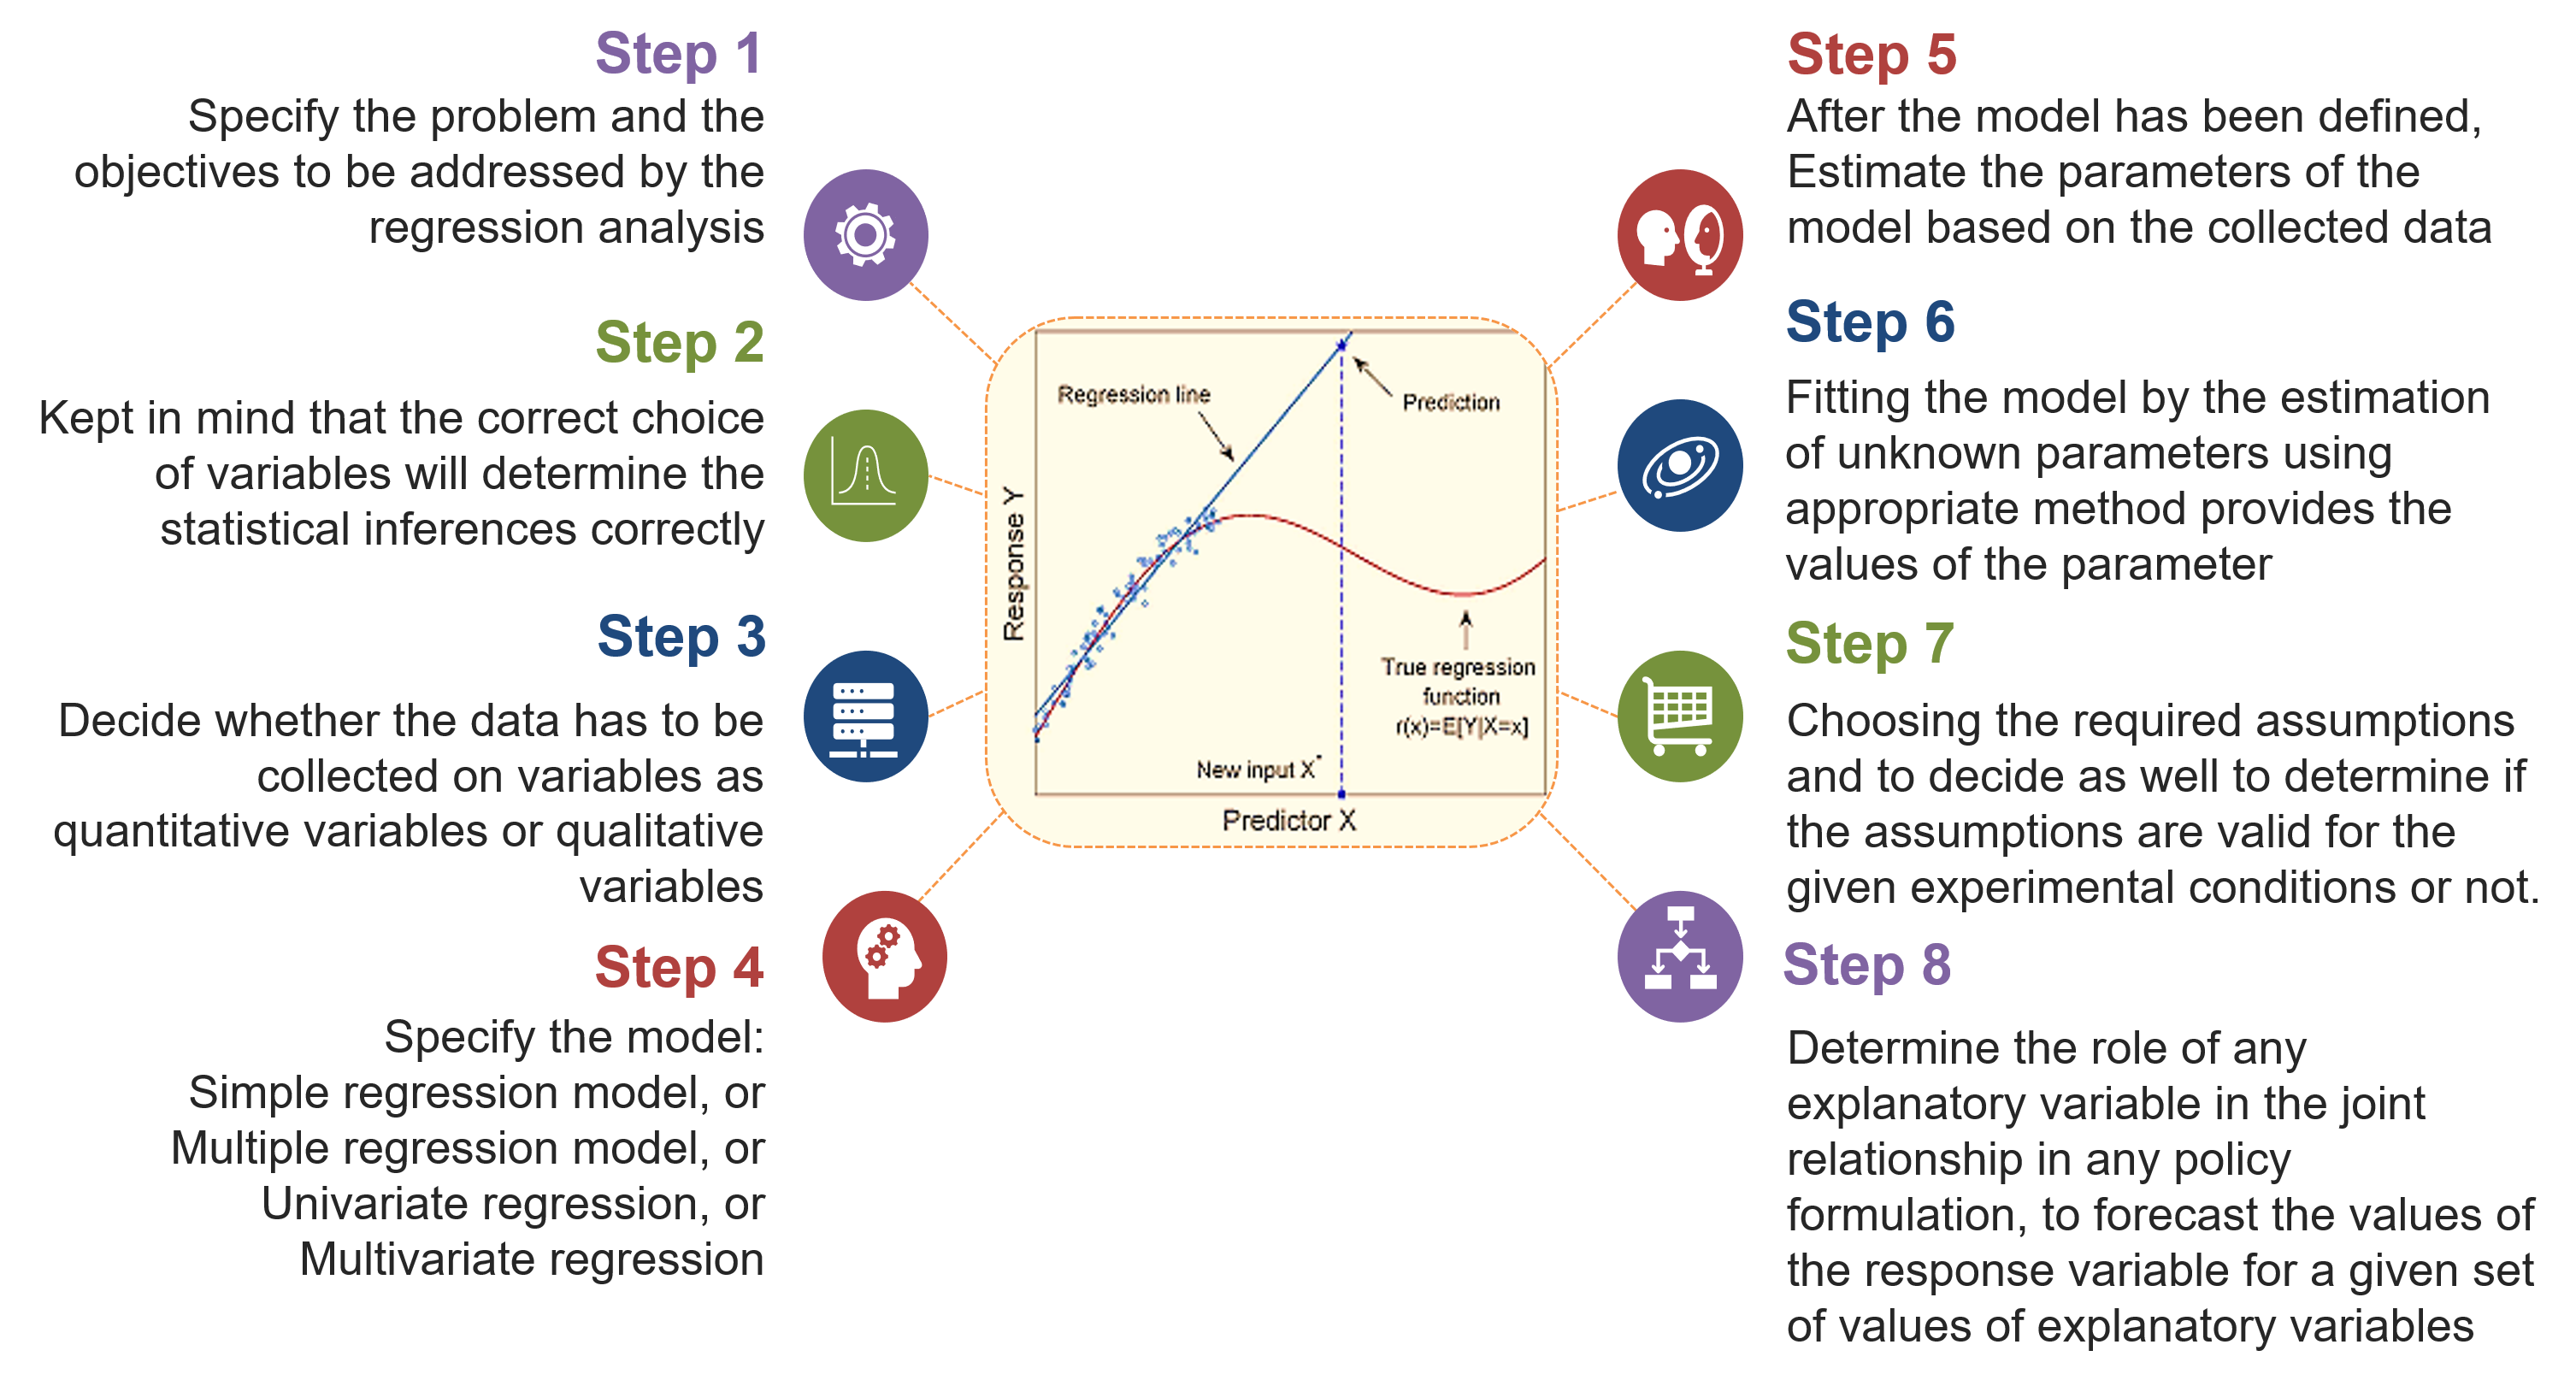
\includegraphics[width=1\linewidth]{images/Bab1/regression} \end{center}

\hypertarget{lab-practicum}{%
\section{Lab Practicum}\label{lab-practicum}}

\hypertarget{simple-regression}{%
\subsection{Simple Regression}\label{simple-regression}}

Suppose you have data on product sales (Y) and advertising costs (X) for several months. Perform a simple regression to understand the relationship between advertising costs and sales. Use the following dataset:

\begin{Shaded}
\begin{Highlighting}[]
\CommentTok{\# Data}
\NormalTok{sales }\OtherTok{\textless{}{-}} \FunctionTok{c}\NormalTok{(}\DecValTok{100}\NormalTok{, }\DecValTok{120}\NormalTok{, }\DecValTok{130}\NormalTok{, }\DecValTok{140}\NormalTok{, }\DecValTok{160}\NormalTok{)}
\NormalTok{advert }\OtherTok{\textless{}{-}} \FunctionTok{c}\NormalTok{(}\DecValTok{50}\NormalTok{, }\DecValTok{70}\NormalTok{, }\DecValTok{90}\NormalTok{, }\DecValTok{110}\NormalTok{, }\DecValTok{130}\NormalTok{)}

\CommentTok{\# Simple Regression Model}
\NormalTok{model1 }\OtherTok{\textless{}{-}} \FunctionTok{lm}\NormalTok{(sales }\SpecialCharTok{\textasciitilde{}}\NormalTok{ advert)}

\CommentTok{\# results}
\FunctionTok{summary}\NormalTok{(model1)}
\end{Highlighting}
\end{Shaded}

\begin{verbatim}
## 
## Call:
## lm(formula = sales ~ advert)
## 
## Residuals:
##         1         2         3         4         5 
## -2.00e+00  4.00e+00 -1.27e-14 -4.00e+00  2.00e+00 
## 
## Coefficients:
##             Estimate Std. Error t value Pr(>|t|)   
## (Intercept)  67.0000     5.4467    12.3   0.0012 **
## advert        0.7000     0.0577    12.1   0.0012 **
## ---
## Signif. codes:  
## 0 '***' 0.001 '**' 0.01 '*' 0.05 '.' 0.1 ' ' 1
## 
## Residual standard error: 3.65 on 3 degrees of freedom
## Multiple R-squared:  0.98,   Adjusted R-squared:  0.973 
## F-statistic:  147 on 1 and 3 DF,  p-value: 0.00121
\end{verbatim}

Based on the regression results above, interpret the regression coefficient, R-squared value, and significance test to see whether advertising costs have a significant influence on sales.

\hypertarget{multiple-regression}{%
\subsection{Multiple Regression}\label{multiple-regression}}

Suppose you have a production dataset that includes production (Y), number of hours worked (X1), and number of machines (X2). Perform multiple regression to model the production relationship with these independent variables.

\begin{Shaded}
\begin{Highlighting}[]
\CommentTok{\# Data}
\NormalTok{product }\OtherTok{\textless{}{-}} \FunctionTok{c}\NormalTok{(}\DecValTok{200}\NormalTok{, }\DecValTok{250}\NormalTok{, }\DecValTok{300}\NormalTok{, }\DecValTok{280}\NormalTok{, }\DecValTok{320}\NormalTok{)}
\NormalTok{work\_hours }\OtherTok{\textless{}{-}} \FunctionTok{c}\NormalTok{(}\DecValTok{40}\NormalTok{, }\DecValTok{50}\NormalTok{, }\DecValTok{60}\NormalTok{, }\DecValTok{55}\NormalTok{, }\DecValTok{65}\NormalTok{)}
\NormalTok{number\_of\_machines }\OtherTok{\textless{}{-}} \FunctionTok{c}\NormalTok{(}\DecValTok{2}\NormalTok{, }\DecValTok{3}\NormalTok{, }\DecValTok{4}\NormalTok{, }\DecValTok{3}\NormalTok{, }\DecValTok{5}\NormalTok{)}

\CommentTok{\# Multiple Regression model}
\NormalTok{model2 }\OtherTok{\textless{}{-}} \FunctionTok{lm}\NormalTok{(product  }\SpecialCharTok{\textasciitilde{}}\NormalTok{ work\_hours }\SpecialCharTok{+}\NormalTok{ number\_of\_machines)}

\CommentTok{\# result}
\FunctionTok{summary}\NormalTok{(model2)}
\end{Highlighting}
\end{Shaded}

\begin{verbatim}
## Warning in summary.lm(model2): essentially perfect
## fit: summary may be unreliable
\end{verbatim}

\begin{verbatim}
## 
## Call:
## lm(formula = product ~ work_hours + number_of_machines)
## 
## Residuals:
##         1         2         3         4         5 
##  2.13e-14 -4.25e-14 -1.43e-17  1.06e-14  1.06e-14 
## 
## Coefficients:
##                     Estimate Std. Error   t value
## (Intercept)        -2.00e+01   1.77e-13 -1.13e+14
## work_hours          6.00e+00   6.36e-15  9.44e+14
## number_of_machines -1.00e+01   5.36e-14 -1.87e+14
##                    Pr(>|t|)    
## (Intercept)          <2e-16 ***
## work_hours           <2e-16 ***
## number_of_machines   <2e-16 ***
## ---
## Signif. codes:  
## 0 '***' 0.001 '**' 0.01 '*' 0.05 '.' 0.1 ' ' 1
## 
## Residual standard error: 3.53e-14 on 2 degrees of freedom
## Multiple R-squared:     1,   Adjusted R-squared:     1 
## F-statistic: 3.54e+30 on 2 and 2 DF,  p-value: <2e-16
\end{verbatim}

Berdasarkan hasil regresi berganda di atas, identifikasi variabel yang memiliki pengaruh signifikan terhadap produksi. Interpretasikan koefisien regresi dan uji signifikan masing-masing variabel.

\hypertarget{catatan}{%
\subsection*{Catatan}\label{catatan}}
\addcontentsline{toc}{subsection}{Catatan}

\begin{itemize}
\tightlist
\item
  Pastikan untuk memberikan penjelasan yang jelas tentang interpretasi hasil, termasuk signifikansi statistik dan koefisien determinasi (R-squared).
\item
  Anda dapat menambahkan visualisasi grafik, seperti plot regresi atau residu, untuk memperjelas analisis.
\item
  Selalu periksa dan pastikan bahwa dataset yang digunakan sesuai dengan konteks soal dan telah diimport dengan benar ke dalam lingkungan R.
\end{itemize}

\hypertarget{simple-regression-1}{%
\chapter{Simple Regression}\label{simple-regression-1}}

\hypertarget{what-is-regression}{%
\section{What is Regression?}\label{what-is-regression}}

Regression is a set of statistical methods used for the estimation of relationships between a dependent variable and one or more independent variables. It can be utilized to assess the strength of the relationship between variables by fitting a line to the observed data. Regression allows you to estimate how the dependent variable changes as the independent variable(s) change. There are several variations of Regression, such as linear, multiple linear, and nonlinear.

The most common models are simple linear and multiple linear. Nonlinear regression analysis is commonly used for more complicated data sets in which the dependent and independent variables show a nonlinear relationship.

\hypertarget{measures-of-the-relationship}{%
\section{Measures Of The Relationship}\label{measures-of-the-relationship}}

There are two quantitative measures of such relationships:

\hypertarget{covariance}{%
\subsection{Covariance}\label{covariance}}

In probability theory and statistics, covariance is a measure of the joint variability of two random variables.

\[
\begin{aligned}
cov(x,y)={\sum^n_{i=1} (x_i-\bar{x})(y_i-\bar{y}) \over n-1} \\
\end{aligned}
\]

Covariance between two variables:

\begin{itemize}
\tightlist
\item
  \(cov(x,y) > 0\), \(x\) and \(y\) tend to move in the same direction
\item
  \(cov(x,y) < 0\), \(x\) and \(y\) tend to move in opposite directions
\item
  \(cov(x,y) = 0\), \(x\) and \(y\) are independent
\end{itemize}

\hypertarget{correlation}{%
\subsection{Correlation}\label{correlation}}

The linear correlation coefficient is also referred to as Pearson's product moment correlation coefficient in honor of Karl Pearson, who originally developed it. This statistic numerically describes how strong the straight-line or linear relationship is between the two variables and the direction, positive or negative.

We can describe the relationship between these two variables graphically and numerically. In order to measure the strength of a linear relationship between two quantitative variables graphically, we use scatter plots:

\begin{center}\includegraphics[width=1\linewidth]{images/Bab2/correlation} \end{center}

If you want to measure the strength of a linear relationship between two quantitative variables numerically, use the following form:

\[
\begin{aligned}
r={cov(x,y)\over s_x s_y}
\end{aligned}
\]

where \(s_x\) are the sample mean and sample standard deviation of the \(x’s\), and \(s_y\) are the mean and standard deviation of the \(y’s.\)

The properties of ``r'':

\begin{itemize}
\tightlist
\item
  It is always between -1 and +1.
\item
  It is a unitless measure so ``r'' would be the same value whether you measured the two variables in pounds and inches or in grams and centimeters.
\item
  Positive values of ``r'' are associated with positive relationships.
\item
  Negative values of ``r'' are associated with negative relationships.
\end{itemize}

\hypertarget{the-general-model}{%
\section{The General Model}\label{the-general-model}}

A simple linear regression model assumes that a linear relationship exists between the conditional expectation of two quantitative variables:

\begin{center}\includegraphics[width=0.8\linewidth]{images/Bab2/linear} \end{center}

where,

\begin{itemize}
\tightlist
\item
  \(Y\) is regarded as the predictor, explanatory, or dependent variable.
\item
  \(X\) is regarded as the response, outcome, or independent variable.
\item
  \(\beta_1\) is the intercept parameter or coefficient
\item
  \(\beta_2\) is the slope parameter or coefficient
\item
  \(\hat{Y}\) is the estimated value of \(Y\) given \(X\)
\item
  \(b_1\) and \(b_2\) is the coefficient estimated value
\end{itemize}

\hypertarget{slr-the-mathematical-model}{%
\subsection{SLR: The Mathematical Model}\label{slr-the-mathematical-model}}

The mathematical representation of a simple linear regression model a model with one dependent variable and only one independent variable can be expressed as:

\[
\begin{aligned}
E(y|x)=\mu_y|x=\beta_1+β_2x
\end{aligned}
\]

where \(\beta_1\) and \(\beta_2\) are the regression parameters that represent the intercept and slope, respectively. We can interpret the above equation as, ``The expected value of the depepndent variable \(y\) given \(x\) is equal to the mean of \(y\) given \(x.\)'' The expected value of \(y\) given \(x,\) according to the equation 3, can be mathematically represented with an intercept \(\beta_1\) and a coefficient of \(x, \beta_2.\) The conditional mean \(E(y|x)\) is called a simple linear regression model because it contains only one non-random independent variable \(x.\)

\hypertarget{slr-the-statistical-model}{%
\subsection{SLR: The Statistical Model}\label{slr-the-statistical-model}}

The simple linear regression model relies on a few assumptions. First, if \(var(y|x)=\sigma^2,\) then the data is said to be homoscedastic. This means that for any value of \(x,\) the variance of \(y\) remains the same. However, this is an unrealistic assumption in real life. Most ``real world data'' that you would be working with will be heteroscedastic, which means that the variance does not remain the same for a given value of \(x.\) The issue of heteroscedasticity is not such a grave sin, depending on the objective and if you have a large enough sample size. However, overcoming this issue is not within the scope of this tutorial. It is just one of the assumptions of the simple linear regression model.

The five assumptions of the simple linear regression model are:

\begin{itemize}
\tightlist
\item
  The mean value of \(y\) for each value of \(x\) is given by the regression function \(E(y|x)=\mu y|x=\beta_1+\beta_2x.\)
\item
  For each value of \(x,\) the values of \(y\) are distributed about their mean value, following the probability distribution that all have the same variance (i.e.~homoscedasticity). That is, \(var(y|x)=\sigma^2.\)
\item
  The sample values of \(y\) are all uncorrelated and have zero covariance, which implies that no linear association exists between them. That is, \(cov(y_i,y_j)=0.\)
\item
  The value \(x\) is not random and must take at least two values.
\item
  (Optional) The values of \(y\) follow a Gaussian Distribution (i.e.~normally distributed about their mean for each value of \(x\)). This means that \(y∼N[\beta_1+\beta_2x,\sigma^2]\)
\end{itemize}

\hypertarget{the-least-squares-principle}{%
\subsection{The Least Squares Principle}\label{the-least-squares-principle}}

The goal in simple linear regression is to estimate the parameters (the \(\beta’s\)). To do so, we must first introduce the least squares principle, the method we will use to estimate these parameters. The \textbf{least squares principle} states that the ``line of best fit'' is the one that minimizes the distance between each point \((x,y)\) to the regression line. In terms of notation, the parameter estimates of \(\beta_1\) and \(\beta_2\) are generally denoted as \(_1\) and \(b_2\), respectively.

The equation for the line of best fit is given by

\[
\begin{aligned}
\hat{y}_i=b_1+b_2x_i
\end{aligned}
\]

The vertical distances between the line of best fit and each point \((x,y)\) are referred to as the \textbf{least squares residuals}, which is given by

\[
\begin{aligned}
\hat{e}_i=y_i−\hat{y}_i=y_i−b_1+b_2x_i
\end{aligned}
\]

In order to find the values for \(b_1\) and \(b_2,\) we want to find the values for the unknown parameters \(\beta_1\) and \(\beta_2\) that minimizes the sum of squares function

\[
\begin{aligned}
S(\beta_1,\beta_2)=\sum_{i=1}^N e^2_i= \biggl(y_i−\beta_1+\beta_2x_i \biggr) ^2
\end{aligned}
\]

The \textbf{least squares estimator} \(b_1\) and \(b_2\) can be solved using the following equations

\[
\begin{aligned}
b_2 & = {\sum^N_{i=1}(x_i−\bar{x})(y_i−\bar{y}) \over \sum^N_{i=1}(x_i−\bar{x})^2 }\\
b_1& = \bar{y}−b_2\bar{x}
\end{aligned}
\]

\hypertarget{least-squares-estimators}{%
\subsection{Least Squares Estimators}\label{least-squares-estimators}}

It is important to note that we may never know the true value of \(\beta_1\) and \(\beta_2,\) and consequently may never know whether our estimates \(b_1\) and \(b_2\) are close to the actual values. The least squares estimates \(\hat{y_i}\) are random variables because they depend on the random variable \(y.\) However, if all of our assumptions hold, then \(E(b_2)=\beta_2\). In a situation where the estimators are equal to their true parameter values, then they are said to be unbiased estimators. If we have a large sample size \(N\) and all of the assumptions for the simple linear regression model hold, then the value of the estimators \(b_1\) and \(b_2\) obtained from all the samples will be \(\beta_1\) and \(\beta_2,\) respectively. The unbiasedness property depends on having many samples of data from the same population.

If all of the assuptions of the linear regression model hold, then the variances and covariances of the estimators are

\[
\begin{aligned}
var(b_1) & =\sigma^2 \biggl[{\sum^n_{i=1}x^2_i \over N(x_i−\bar{x})^2}\biggl] \\
var(b_2) & ={\sigma^2 \over \sum(x_i−\bar{x})^2}  \\
cov(b_1,b_2) & =\sigma^2 \biggl[{−\bar{x} \over ∑^n_{i=1}(x_i−\bar{x})^2}\biggr] \\
\end{aligned}
\]

The variance of an estimator measures the precision of the estimator in the sense that it tells us how much the estimates can vary from sample to sample. \textbf{\emph{The smaller the variance, the greater the sampling precision}}. Then the Gauss-Markov Theorem states that the estimators \(b_1\) and \(b_2\) have the smallest variance of all linear and unbiased estimators of \(\beta_1\) and \(\beta_2.\) Such estimators are commonly referred to as the best linear unbiased estimator (BLUE).

\hypertarget{estimate-the-var-and-cov}{%
\subsection{Estimate the Var and Cov}\label{estimate-the-var-and-cov}}

Recall that the variance of the random error term \(e\) is

\[
\begin{aligned}
var(e_i)=E\biggl[e_i−E(e_i)\biggr]^2
\end{aligned}
\]

If the assumption \(E(e_i)=0.\) If the assumption holds, we can then rewrite the variance of the random error term \(e\) as

\[
\begin{aligned}
var(e_i)=\sigma^2=E[e_i]^2={1\over N} \sum_{i=1}^N e^2_i
\end{aligned}
\]

Unfortunately, the above formula is of little to no use since the random error term \(e_i\) is unobservable. Fortunately, since \(e_i=y_i−E(y|x)=y_i−\beta1+\beta_2x_i,\) we can replace the unknown parameters \(\beta_1\) and \(\beta_2\) with their least squares estimates \(b_1\) and \(b_2\) to obtain

\[
\begin{aligned}
\hat{e}_i=y_i−\hat{y}_i=y_i−b_1+b_2x_i
\end{aligned}
\]

The unbiased estimator of the variance of the random error term is

\[
\begin{aligned}
\sigma^2={\sum \hat{e}_i \over N−2}
\end{aligned}
\]

where 2 represents the number of parameters (in this case \(\beta_1\) and \(\beta_2\)). We refer to this as having \(N−2\) degrees of freedom. Now that we have an unbiased estimator of the variance of our random error term \(e,\) we can estimate the variances and covarianes of their least squares estimates.

\[
\begin{aligned}
\widehat{var(b_1)} & = \hat{\sigma^2} \biggl[{\sum^n_{i=1}x^2_i \over N(x_i−\bar{x})^2}\biggl] \\
\widehat{var(b_2)} & ={\hat{\sigma^2} \over \sum(x_i−\bar{x})^2}  \\
\widehat{cov(b_1,b_2)} & = \hat{\sigma^2} \biggl[{−\bar{x} \over ∑^n_{i=1}(x_i−\bar{x})^2}\biggr] \\
\end{aligned}
\]

\hypertarget{lab-practicum-1}{%
\section{Lab Practicum}\label{lab-practicum-1}}

The data for this example is stored in the R package \texttt{PoEdata}. First, you have to install the ``PoEdata'' package, type the following script lines in the Console window of RStudio:

\begin{Shaded}
\begin{Highlighting}[]
\CommentTok{\# install.packages("remotes")}
\CommentTok{\# remotes::install\_github("ccolonescu/PoEdata")}
\end{Highlighting}
\end{Shaded}

Then, consider the data set:

\begin{Shaded}
\begin{Highlighting}[]
\FunctionTok{library}\NormalTok{(PoEdata)                                     }\CommentTok{\# load the library PoEdata}
\FunctionTok{library}\NormalTok{(DT)                                          }\CommentTok{\# use for datatable fuction }
\FunctionTok{data}\NormalTok{(}\StringTok{"food"}\NormalTok{, }\AttributeTok{package=}\StringTok{"PoEdata"}\NormalTok{)}
\FunctionTok{datatable}\NormalTok{(food)}
\end{Highlighting}
\end{Shaded}

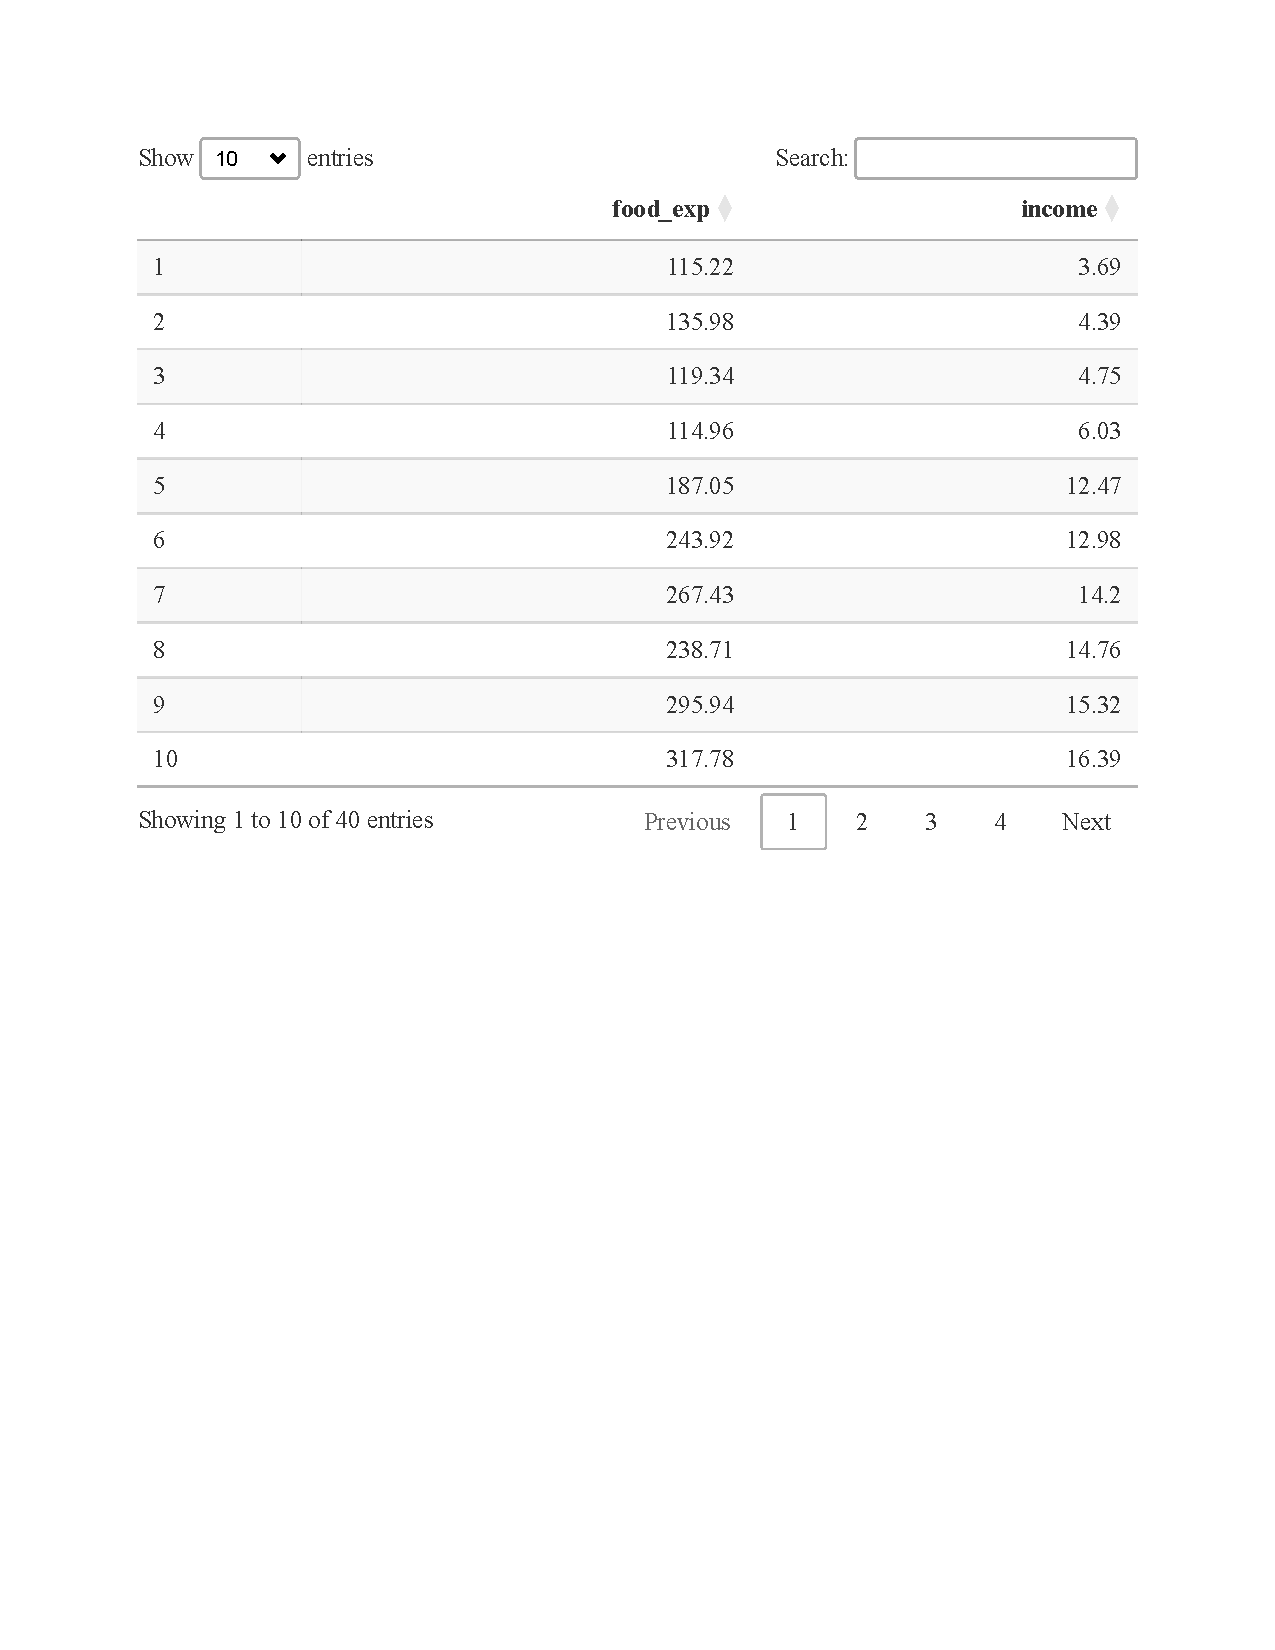
\includegraphics{Econometrics_files/figure-latex/unnamed-chunk-4-1.pdf}

It is always a good idea to visually inspect the data in a scatter diagram, which can be created using the function \texttt{plot()}. The figure bellow is a scatter diagram of food expenditure on income, suggesting that there is a positive relationship between income and food expenditure.

\begin{Shaded}
\begin{Highlighting}[]
\FunctionTok{plot}\NormalTok{(food}\SpecialCharTok{$}\NormalTok{income, food}\SpecialCharTok{$}\NormalTok{food\_exp, }
     \AttributeTok{ylim=}\FunctionTok{c}\NormalTok{(}\DecValTok{0}\NormalTok{, }\FunctionTok{max}\NormalTok{(food}\SpecialCharTok{$}\NormalTok{food\_exp)),}
     \AttributeTok{xlim=}\FunctionTok{c}\NormalTok{(}\DecValTok{0}\NormalTok{, }\FunctionTok{max}\NormalTok{(food}\SpecialCharTok{$}\NormalTok{income)),}
     \AttributeTok{xlab=}\StringTok{"weekly income in $100"}\NormalTok{, }
     \AttributeTok{ylab=}\StringTok{"weekly food expenditure in $"}\NormalTok{, }
     \AttributeTok{type =} \StringTok{"p"}\NormalTok{)}
\end{Highlighting}
\end{Shaded}

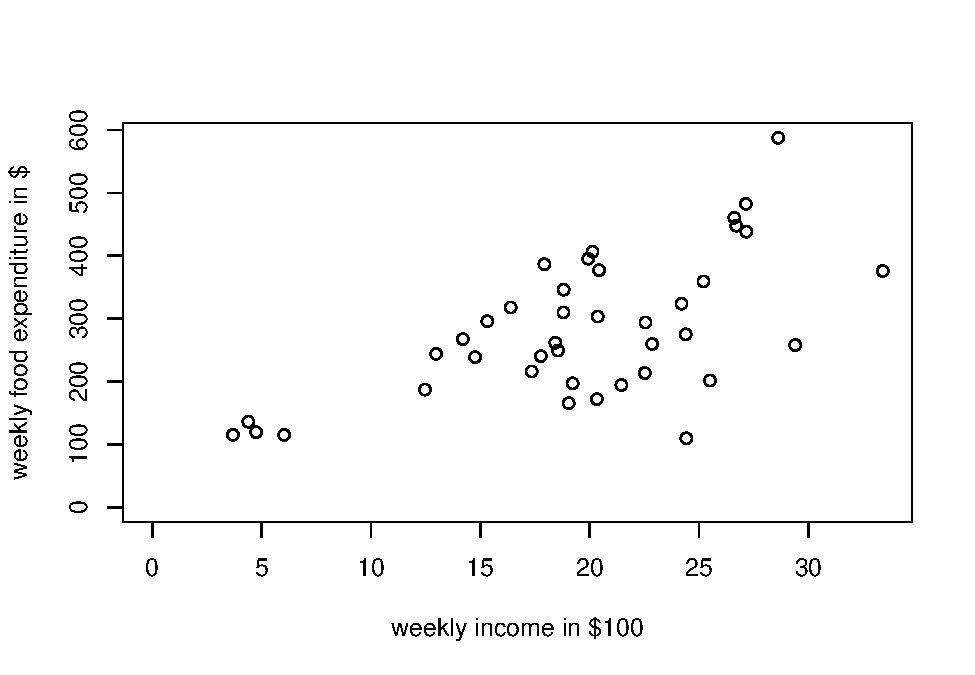
\includegraphics{Econometrics_files/figure-latex/unnamed-chunk-5-1.pdf}

\href{https://www.investopedia.com/terms/r/r-squared.asp}{About \(R^2\)}

\hypertarget{estimating-a-linear-regression}{%
\subsection{Estimating a Linear Regression}\label{estimating-a-linear-regression}}

For the food expenditure data, the regression model will be

\[
\begin{aligned}
Y&=\beta_1+\beta_2 *X+e \\
food_{exp}&=\beta_1+\beta_2*income+e
\end{aligned}
\]

The R function for estimating a linear regression model is \texttt{lm(y\textasciitilde{}x,\ data)} which, used just by itself does not show any output; It is useful to give the model a name, such as \texttt{mod1}, then show the results using \texttt{summary(mod1)}.

\begin{Shaded}
\begin{Highlighting}[]
\NormalTok{mod1 }\OtherTok{\textless{}{-}} \FunctionTok{lm}\NormalTok{(food\_exp }\SpecialCharTok{\textasciitilde{}}\NormalTok{ income, }\AttributeTok{data =}\NormalTok{ food)           }\CommentTok{\# linear model}
\NormalTok{smod1}\OtherTok{\textless{}{-}} \FunctionTok{summary}\NormalTok{(mod1)                                }\CommentTok{\# get summary }
\NormalTok{smod1}
\end{Highlighting}
\end{Shaded}

\begin{verbatim}
## 
## Call:
## lm(formula = food_exp ~ income, data = food)
## 
## Residuals:
##     Min      1Q  Median      3Q     Max 
## -223.03  -50.82   -6.32   67.88  212.04 
## 
## Coefficients:
##             Estimate Std. Error t value Pr(>|t|)    
## (Intercept)    83.42      43.41    1.92    0.062 .  
## income         10.21       2.09    4.88  1.9e-05 ***
## ---
## Signif. codes:  
## 0 '***' 0.001 '**' 0.01 '*' 0.05 '.' 0.1 ' ' 1
## 
## Residual standard error: 89.5 on 38 degrees of freedom
## Multiple R-squared:  0.385,  Adjusted R-squared:  0.369 
## F-statistic: 23.8 on 1 and 38 DF,  p-value: 1.95e-05
\end{verbatim}

If you are interested in only some of the results of the regression, such as the estimated coefficients, you can retrieve them using specific functions, such as the function \texttt{coef()}.

\begin{Shaded}
\begin{Highlighting}[]
\NormalTok{b1 }\OtherTok{\textless{}{-}} \FunctionTok{coef}\NormalTok{(mod1)[[}\DecValTok{1}\NormalTok{]]                                }\CommentTok{\# the estimated value of  β1}
\NormalTok{b2 }\OtherTok{\textless{}{-}} \FunctionTok{coef}\NormalTok{(mod1)[[}\DecValTok{2}\NormalTok{]]                                }\CommentTok{\# the estimated value of  β2}
\NormalTok{b1}
\end{Highlighting}
\end{Shaded}

\begin{verbatim}
## [1] 83.42
\end{verbatim}

\begin{Shaded}
\begin{Highlighting}[]
\NormalTok{b2}
\end{Highlighting}
\end{Shaded}

\begin{verbatim}
## [1] 10.21
\end{verbatim}

From the result, we can write our estimating linear regression as:

\[
\begin{aligned}
\hat{Y}&=b_1+b_2*X \\
\hat{food_{exp}}&=83.416+10.20964*income
\end{aligned}
\]

The intercept parameter, \(\beta_1\) , is usually of little importance in econometric models; we are mostly interested in the slope parameter, \(\beta_2\). The estimated value of \(\beta_2\) suggests that the food expenditure for an average family increases by 10.209643 when the family income increases by 1 unit, which in this case is \$100. The R function \texttt{abline()} adds the \texttt{regfression} line to the previously plotted scatter diagram bellow:

\begin{Shaded}
\begin{Highlighting}[]
\FunctionTok{plot}\NormalTok{(food}\SpecialCharTok{$}\NormalTok{income, food}\SpecialCharTok{$}\NormalTok{food\_exp, }
     \AttributeTok{xlab=}\StringTok{"weekly income in $100"}\NormalTok{, }
     \AttributeTok{ylab=}\StringTok{"weekly food expenditure in $"}\NormalTok{, }
     \AttributeTok{type =} \StringTok{"p"}\NormalTok{)}
\FunctionTok{abline}\NormalTok{(b1,b2)}
\end{Highlighting}
\end{Shaded}

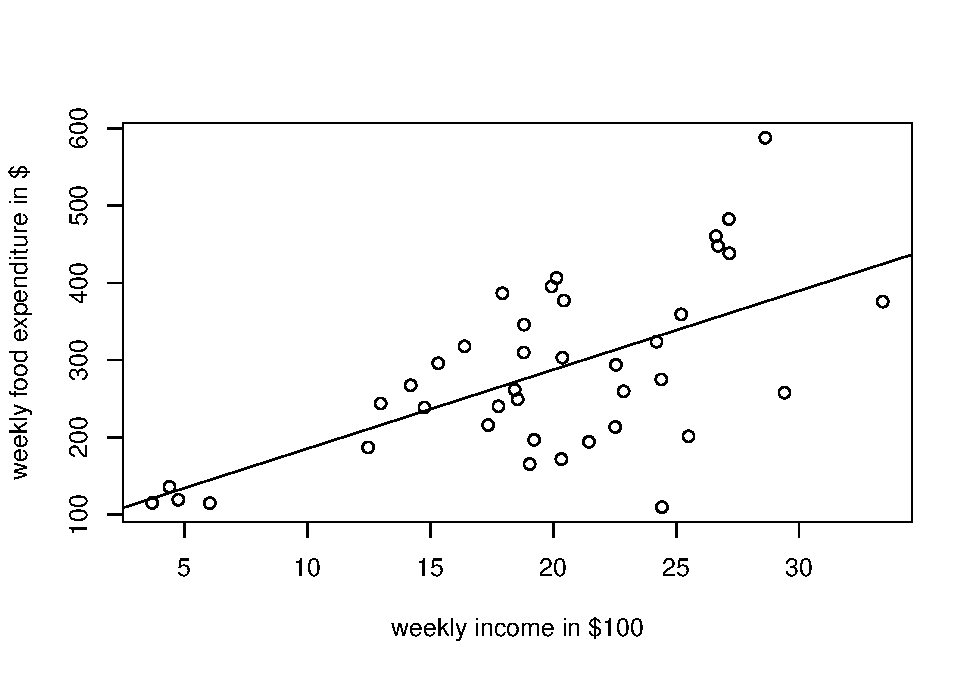
\includegraphics{Econometrics_files/figure-latex/unnamed-chunk-8-1.pdf}

How can one retrieve various regression results? To retrieve a particular result you just refer to it with the name of the object, followed by the \$ sign and the name of the result you wish to retrieve. For instance, if we want the vector of coefficients from \texttt{mod1}, we refer to it as \texttt{mod1\textbackslash{}\$coefficients} and \texttt{smod1\textbackslash{}\$coefficients}:

\begin{Shaded}
\begin{Highlighting}[]
\NormalTok{mod1}\SpecialCharTok{$}\NormalTok{coefficients}
\end{Highlighting}
\end{Shaded}

\begin{verbatim}
## (Intercept)      income 
##       83.42       10.21
\end{verbatim}

\begin{Shaded}
\begin{Highlighting}[]
\NormalTok{smod1}\SpecialCharTok{$}\NormalTok{coefficients}
\end{Highlighting}
\end{Shaded}

\begin{verbatim}
##             Estimate Std. Error t value  Pr(>|t|)
## (Intercept)    83.42     43.410   1.922 6.218e-02
## income         10.21      2.093   4.877 1.946e-05
\end{verbatim}

\begin{Shaded}
\begin{Highlighting}[]
\FunctionTok{names}\NormalTok{(mod1)                                          }\CommentTok{\# for more}
\FunctionTok{names}\NormalTok{(smod1)                                         }\CommentTok{\# for more}
\end{Highlighting}
\end{Shaded}

As we have seen before, however, some of these results can be retrieved using specific functions, such as \texttt{coef(mod1),\ resid(mod1),\ fitted(mod1),\ and\ vcov(mod1)}.

\begin{center}\rule{0.5\linewidth}{0.5pt}\end{center}

\hypertarget{prediction-with-slr-model}{%
\subsection{Prediction with SLR Model}\label{prediction-with-slr-model}}

The estimated regression parameters, \(b_1\) and \(b_2\) allow us to predict the expected food expenditure for any given income. All we need to do is to plug the estimated parameter values and the given income into an equation like Equation 15 . For example, the expected value of \texttt{food\_exp} for an income of \$2000 is calculated in Equation 16 . (Remember to divide the income by 100, since the data for the variable income is in hundreds of dollars.)

\[
\begin{aligned}
\hat{food_{exp}}&=83.416+10.20964*20\\
& = $ 287.608861
\end{aligned}
\]

R, however, does this calculations for us with its function called \texttt{predict()}. Let us extend slightly the example to more than one income for which we predict food expenditure, say income = \$2000, \$2500, and \$2700. The function \texttt{predict()} in R requires that the new values of the independent variables be organized under a particular form, called a data frame. Even when we only want to predict for one income, we need the same data-frame structure. In R, a set of numbers is held together using the structure \texttt{c()}. The following sequence shows this example.

\begin{Shaded}
\begin{Highlighting}[]
\NormalTok{mod1 }\OtherTok{\textless{}{-}} \FunctionTok{lm}\NormalTok{(food\_exp}\SpecialCharTok{\textasciitilde{}}\NormalTok{income, }\AttributeTok{data=}\NormalTok{food)}
\NormalTok{newx }\OtherTok{\textless{}{-}} \FunctionTok{data.frame}\NormalTok{(}\AttributeTok{income =} \FunctionTok{c}\NormalTok{(}\DecValTok{20}\NormalTok{, }\DecValTok{25}\NormalTok{, }\DecValTok{27}\NormalTok{))}
\NormalTok{yhat }\OtherTok{\textless{}{-}} \FunctionTok{predict}\NormalTok{(mod1, newx)}
\NormalTok{yhat                                                 }\CommentTok{\# prints the result}
\end{Highlighting}
\end{Shaded}

\begin{verbatim}
##     1     2     3 
## 287.6 338.7 359.1
\end{verbatim}

\begin{center}\rule{0.5\linewidth}{0.5pt}\end{center}

\hypertarget{assess-regression-coefficients}{%
\subsection{Assess Regression Coefficients}\label{assess-regression-coefficients}}

The regression coefficients \(b_1\) and \(b_2\) are random variables, because they depend on sample. In this case, we repeated samples to assess regression coefficients. Let us construct a number of random subsamples from the food data and re-calculate \(b_1\) and \(b_2\) . A random subsample can be constructed using the function \texttt{sample()}, as the following example illustrates only for \(b_2\).

\begin{Shaded}
\begin{Highlighting}[]
\NormalTok{N }\OtherTok{\textless{}{-}} \FunctionTok{nrow}\NormalTok{(food)   }\CommentTok{\# returns the number of observations in the dataset}
\NormalTok{C }\OtherTok{\textless{}{-}} \DecValTok{50}           \CommentTok{\# desired number of subsamples}
\NormalTok{S }\OtherTok{\textless{}{-}} \DecValTok{38}           \CommentTok{\# desired sample size}

\NormalTok{sumb2 }\OtherTok{\textless{}{-}} \DecValTok{0}
\ControlFlowTok{for}\NormalTok{ (i }\ControlFlowTok{in} \DecValTok{1}\SpecialCharTok{:}\NormalTok{C)\{   }\CommentTok{\# a loop over the number of subsamples}
  \FunctionTok{set.seed}\NormalTok{(}\DecValTok{3}\SpecialCharTok{*}\NormalTok{i)   }\CommentTok{\# a different seed for each subsample  }
\NormalTok{  subsample }\OtherTok{\textless{}{-}}\NormalTok{ food[}\FunctionTok{sample}\NormalTok{(}\DecValTok{1}\SpecialCharTok{:}\NormalTok{N, }\AttributeTok{size=}\NormalTok{S, }\AttributeTok{replace=}\ConstantTok{TRUE}\NormalTok{), ]}
\NormalTok{  mod2 }\OtherTok{\textless{}{-}} \FunctionTok{lm}\NormalTok{(food\_exp}\SpecialCharTok{\textasciitilde{}}\NormalTok{income, }\AttributeTok{data=}\NormalTok{subsample)}
  \CommentTok{\#sum b2 for all subsamples:}
\NormalTok{  sumb2 }\OtherTok{\textless{}{-}}\NormalTok{ sumb2 }\SpecialCharTok{+} \FunctionTok{coef}\NormalTok{(mod2)[[}\DecValTok{2}\NormalTok{]]}
\NormalTok{\}}
\FunctionTok{print}\NormalTok{(sumb2}\SpecialCharTok{/}\NormalTok{C, }\AttributeTok{digits =} \DecValTok{3}\NormalTok{)}
\end{Highlighting}
\end{Shaded}

\begin{verbatim}
## [1] 9.89
\end{verbatim}

The result, \(b_2=9.88\), is the average of 50 estimates of \(b_2\).

\begin{center}\rule{0.5\linewidth}{0.5pt}\end{center}

\hypertarget{estimated-var-and-cov}{%
\subsection{Estimated Var and Cov}\label{estimated-var-and-cov}}

Many applications require estimates of the variances and covariances of the regression coefficients. R stores them in the a matrix \texttt{vcov()}:

\begin{Shaded}
\begin{Highlighting}[]
\NormalTok{(varb1 }\OtherTok{\textless{}{-}} \FunctionTok{vcov}\NormalTok{(mod1)[}\DecValTok{1}\NormalTok{, }\DecValTok{1}\NormalTok{])}
\end{Highlighting}
\end{Shaded}

\begin{verbatim}
## [1] 1884
\end{verbatim}

\begin{Shaded}
\begin{Highlighting}[]
\NormalTok{(varb2 }\OtherTok{\textless{}{-}} \FunctionTok{vcov}\NormalTok{(mod1)[}\DecValTok{2}\NormalTok{, }\DecValTok{2}\NormalTok{])}
\end{Highlighting}
\end{Shaded}

\begin{verbatim}
## [1] 4.382
\end{verbatim}

\begin{Shaded}
\begin{Highlighting}[]
\NormalTok{(covb1b2 }\OtherTok{\textless{}{-}} \FunctionTok{vcov}\NormalTok{(mod1)[}\DecValTok{1}\NormalTok{,}\DecValTok{2}\NormalTok{])}
\end{Highlighting}
\end{Shaded}

\begin{verbatim}
## [1] -85.9
\end{verbatim}

\hypertarget{non-linear-relationships}{%
\subsection{Non-Linear Relationships}\label{non-linear-relationships}}

Sometimes the scatter plot diagram or some theoretical consideraions suggest a non-linear relationship. The most popular non-linear relationships involve logarithms of the dependent or independent variables and polinomial functions. The quadratic model requires the square of the independent variable.

\[
\begin{aligned}
Y=\beta_1+\beta_2*X^2+e\\
\end{aligned}
\]
In R, independent variables involving mathematical operators can be included in a regression equation with the function \texttt{I()}. The following example uses the dataset br from the package \texttt{PoEdata}, which includes the sale prices and the attributes of 1080 houses in Baton Rouge, LA. price is the sale price in dollars, and sqft is the surface area in square feet.

\begin{Shaded}
\begin{Highlighting}[]
\FunctionTok{data}\NormalTok{(br)}
\NormalTok{mod2 }\OtherTok{\textless{}{-}} \FunctionTok{lm}\NormalTok{(price}\SpecialCharTok{\textasciitilde{}}\FunctionTok{I}\NormalTok{(sqft}\SpecialCharTok{\^{}}\DecValTok{2}\NormalTok{), }\AttributeTok{data=}\NormalTok{br)}
\NormalTok{b1 }\OtherTok{\textless{}{-}} \FunctionTok{coef}\NormalTok{(mod2)[[}\DecValTok{1}\NormalTok{]]}
\NormalTok{b2 }\OtherTok{\textless{}{-}} \FunctionTok{coef}\NormalTok{(mod2)[[}\DecValTok{2}\NormalTok{]]}
\NormalTok{sqftx}\OtherTok{=}\FunctionTok{c}\NormalTok{(}\DecValTok{2000}\NormalTok{, }\DecValTok{4000}\NormalTok{, }\DecValTok{6000}\NormalTok{)            }\CommentTok{\# given values for sqft}
\NormalTok{pricex}\OtherTok{=}\NormalTok{b1}\SpecialCharTok{+}\NormalTok{b2}\SpecialCharTok{*}\NormalTok{sqftx}\SpecialCharTok{\^{}}\DecValTok{2}                 \CommentTok{\# prices corresponding to given sqft }
\NormalTok{DpriceDsqft }\OtherTok{\textless{}{-}} \DecValTok{2}\SpecialCharTok{*}\NormalTok{b2}\SpecialCharTok{*}\NormalTok{sqftx            }\CommentTok{\# marginal effect of sqft on price}
\NormalTok{elasticity}\OtherTok{=}\NormalTok{DpriceDsqft}\SpecialCharTok{*}\NormalTok{sqftx}\SpecialCharTok{/}\NormalTok{pricex }
\NormalTok{b1; b2; DpriceDsqft; elasticity      }\CommentTok{\# prints results}
\end{Highlighting}
\end{Shaded}

\begin{verbatim}
## [1] 55777
\end{verbatim}

\begin{verbatim}
## [1] 0.01542
\end{verbatim}

\begin{verbatim}
## [1]  61.69 123.37 185.06
\end{verbatim}

\begin{verbatim}
## [1] 1.050 1.631 1.817
\end{verbatim}

We woud like now to draw a scatter diagram and see how the quadratic function fits the data. The next chunk of code provides two alternatives for constructing such a graph. The first simply draws the quadratic function on the scatter diagram, using the R function \texttt{curve()}; the second uses the function lines, which requires ordering the data set in increasing values of \texttt{sqft} before the regression model is evaluated, such that the resulting fitted values will also come out in the same order.

\begin{Shaded}
\begin{Highlighting}[]
\FunctionTok{plot}\NormalTok{(br}\SpecialCharTok{$}\NormalTok{sqft, br}\SpecialCharTok{$}\NormalTok{price, }\AttributeTok{xlab=}\StringTok{"Total square feet"}\NormalTok{, }
     \AttributeTok{ylab=}\StringTok{"Sale price, $"}\NormalTok{, }\AttributeTok{col=}\StringTok{"grey"}\NormalTok{)}
\CommentTok{\#add the quadratic curve to the scatter plot:}
\FunctionTok{curve}\NormalTok{(b1}\SpecialCharTok{+}\NormalTok{b2}\SpecialCharTok{*}\NormalTok{x}\SpecialCharTok{\^{}}\DecValTok{2}\NormalTok{, }\AttributeTok{col=}\StringTok{"red"}\NormalTok{, }\AttributeTok{add=}\ConstantTok{TRUE}\NormalTok{) }
\end{Highlighting}
\end{Shaded}

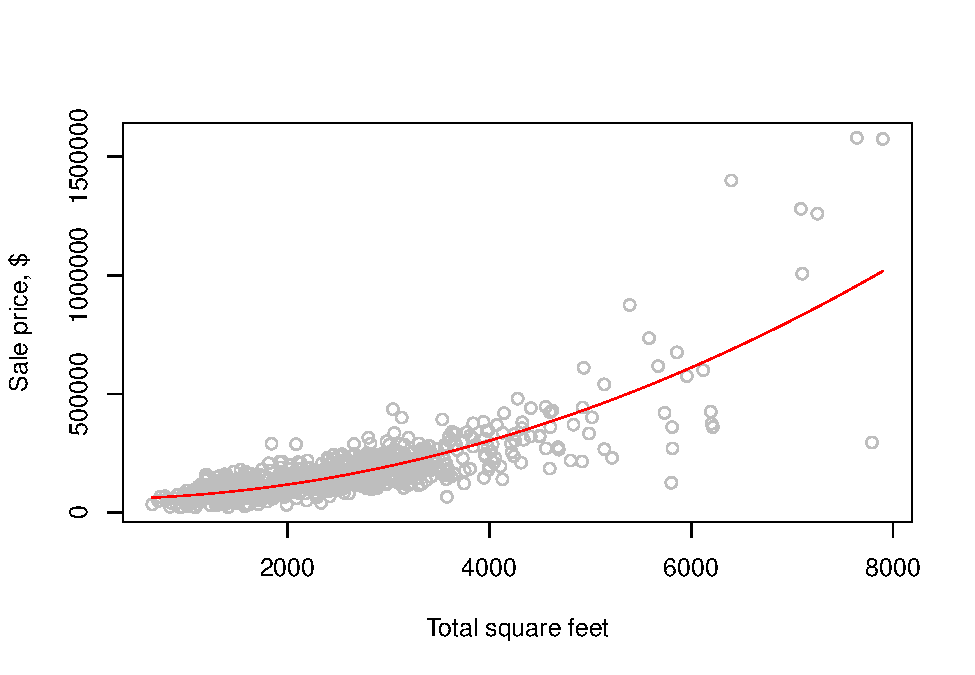
\includegraphics{Econometrics_files/figure-latex/unnamed-chunk-16-1.pdf}

An alternative way to draw the fitted curve:

\begin{Shaded}
\begin{Highlighting}[]
\NormalTok{ordat }\OtherTok{\textless{}{-}}\NormalTok{ br[}\FunctionTok{order}\NormalTok{(br}\SpecialCharTok{$}\NormalTok{sqft), ] }\CommentTok{\#sorts the dataset after \textasciigrave{}sqft\textasciigrave{}}
\NormalTok{mod2 }\OtherTok{\textless{}{-}} \FunctionTok{lm}\NormalTok{(price}\SpecialCharTok{\textasciitilde{}}\FunctionTok{I}\NormalTok{(sqft}\SpecialCharTok{\^{}}\DecValTok{2}\NormalTok{), }\AttributeTok{data=}\NormalTok{ordat)}
\FunctionTok{plot}\NormalTok{(br}\SpecialCharTok{$}\NormalTok{sqft, br}\SpecialCharTok{$}\NormalTok{price, }
     \AttributeTok{main=}\StringTok{"Dataset ordered after \textquotesingle{}sqft\textquotesingle{} "}\NormalTok{, }
     \AttributeTok{xlab=}\StringTok{"Total square feet"}\NormalTok{, }
     \AttributeTok{ylab=}\StringTok{"Sale price, $"}\NormalTok{, }\AttributeTok{col=}\StringTok{"grey"}\NormalTok{)}
\FunctionTok{lines}\NormalTok{(}\FunctionTok{fitted}\NormalTok{(mod31)}\SpecialCharTok{\textasciitilde{}}\NormalTok{ordat}\SpecialCharTok{$}\NormalTok{sqft, }\AttributeTok{col=}\StringTok{"red"}\NormalTok{)}
\end{Highlighting}
\end{Shaded}

The log-linear model regresses the log of the dependent variable on a linear expression of the independent variable (unless otherwise specified, the log notation stands for natural logarithm, following a usual convention in economics):

\[
\begin{aligned}
Log(Y)=\beta_1+\beta_2*X+e\\
\end{aligned}
\]

One of the reasons to use the log of an independent variable is to make its distribution closer to the normal distribution. Let us draw the histograms of price and log(price) to compare them

\begin{Shaded}
\begin{Highlighting}[]
\FunctionTok{hist}\NormalTok{(br}\SpecialCharTok{$}\NormalTok{price, }\AttributeTok{col=}\StringTok{\textquotesingle{}grey\textquotesingle{}}\NormalTok{)}
\end{Highlighting}
\end{Shaded}

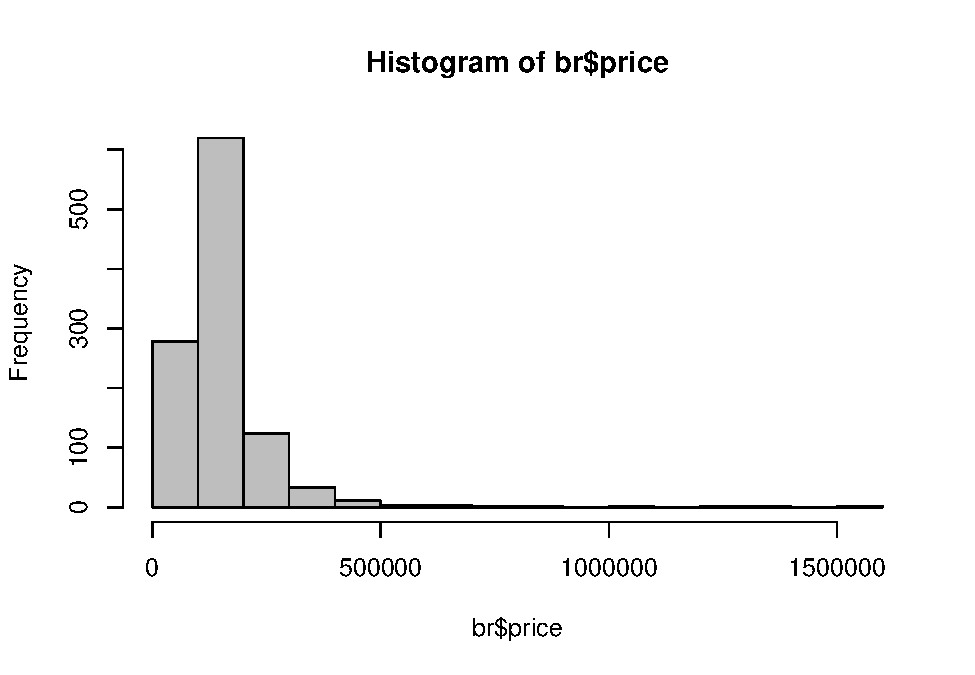
\includegraphics{Econometrics_files/figure-latex/unnamed-chunk-18-1.pdf}

\begin{Shaded}
\begin{Highlighting}[]
\FunctionTok{hist}\NormalTok{(}\FunctionTok{log}\NormalTok{(br}\SpecialCharTok{$}\NormalTok{price), }\AttributeTok{col=}\StringTok{\textquotesingle{}grey\textquotesingle{}}\NormalTok{)}
\end{Highlighting}
\end{Shaded}

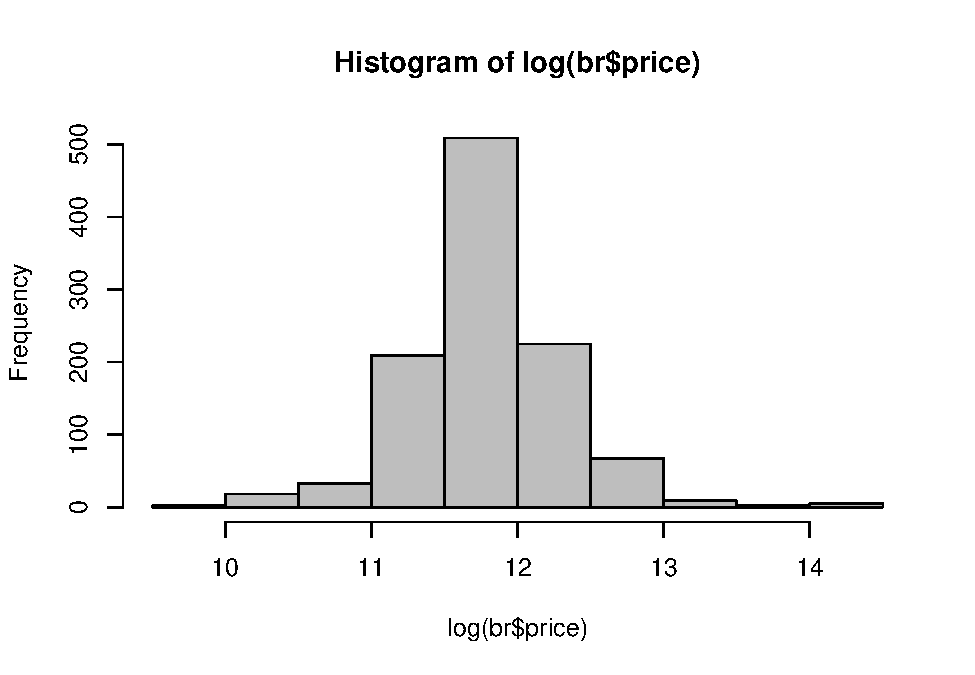
\includegraphics{Econometrics_files/figure-latex/unnamed-chunk-18-2.pdf}

We are interested, as before, in the estimates of the coefficients and their interpretation, in the fitted values of price, and in the marginal effect of an increase in sqft on price.

\begin{Shaded}
\begin{Highlighting}[]
\NormalTok{mod3 }\OtherTok{\textless{}{-}} \FunctionTok{lm}\NormalTok{(}\FunctionTok{log}\NormalTok{(price)}\SpecialCharTok{\textasciitilde{}}\NormalTok{sqft, }\AttributeTok{data=}\NormalTok{br)}
\NormalTok{mod3}\SpecialCharTok{$}\NormalTok{coefficients}
\end{Highlighting}
\end{Shaded}

\begin{verbatim}
## (Intercept)        sqft 
##   1.084e+01   4.113e-04
\end{verbatim}

The coefficients are \(b_1= 10.84\) and \(b_2= 0.00041\), showing that an increase in the surface area (sqft) of an apartment by one unit (1 sqft) increases the price of the apartment by 0.041 percent. Thus, for a house price of \$100,000, an increase of 100 sqft will increase the price by approximately 100∗0.041 percent, which is equal to \$4112.7. In general, the marginal effect of an increase in \(X\) on \(Y\) in Equation 19 is

\[
\begin{aligned}
{dy\over dx}=\beta_2 * Y
\end{aligned}
\]

and the elasticity is

\[
\begin{aligned}
e= {dy\over dx} {X\over Y}=\beta_2 * X
\end{aligned}
\]

The next lines of code show how to draw the fitted values curve of the loglinear model and how to calculate the marginal effect and the elasticity for the median price in the dataset. The fitted values are here calculated using the formula

\[
\begin{aligned}
\hat{Y}= e^{b_1+b_2*X}
\end{aligned}
\]

\begin{Shaded}
\begin{Highlighting}[]
\NormalTok{ordat }\OtherTok{\textless{}{-}}\NormalTok{ br[}\FunctionTok{order}\NormalTok{(br}\SpecialCharTok{$}\NormalTok{sqft), ] }\CommentTok{\#order the dataset}
\NormalTok{mod4 }\OtherTok{\textless{}{-}} \FunctionTok{lm}\NormalTok{(}\FunctionTok{log}\NormalTok{(price)}\SpecialCharTok{\textasciitilde{}}\NormalTok{sqft, }\AttributeTok{data=}\NormalTok{ordat)}
\FunctionTok{plot}\NormalTok{(br}\SpecialCharTok{$}\NormalTok{sqft, br}\SpecialCharTok{$}\NormalTok{price, }\AttributeTok{col=}\StringTok{"grey"}\NormalTok{)}
\FunctionTok{lines}\NormalTok{(}\FunctionTok{exp}\NormalTok{(}\FunctionTok{fitted}\NormalTok{(mod4))}\SpecialCharTok{\textasciitilde{}}\NormalTok{ordat}\SpecialCharTok{$}\NormalTok{sqft, }
      \AttributeTok{col=}\StringTok{"blue"}\NormalTok{, }\AttributeTok{main=}\StringTok{"Log{-}linear Model"}\NormalTok{)}
\end{Highlighting}
\end{Shaded}

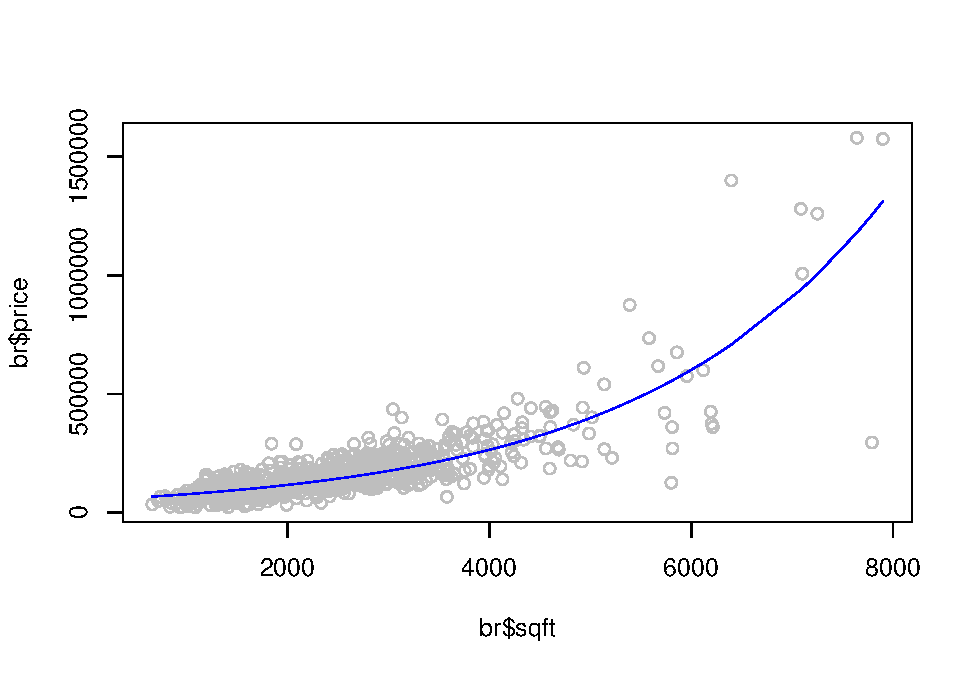
\includegraphics{Econometrics_files/figure-latex/unnamed-chunk-20-1.pdf}

\begin{Shaded}
\begin{Highlighting}[]
\NormalTok{pricex}\OtherTok{\textless{}{-}} \FunctionTok{median}\NormalTok{(br}\SpecialCharTok{$}\NormalTok{price)}
\NormalTok{sqftx }\OtherTok{\textless{}{-}}\NormalTok{ (}\FunctionTok{log}\NormalTok{(pricex)}\SpecialCharTok{{-}}\FunctionTok{coef}\NormalTok{(mod4)[[}\DecValTok{1}\NormalTok{]])}\SpecialCharTok{/}\FunctionTok{coef}\NormalTok{(mod4)[[}\DecValTok{2}\NormalTok{]]}
\NormalTok{(DyDx }\OtherTok{\textless{}{-}}\NormalTok{ pricex}\SpecialCharTok{*}\FunctionTok{coef}\NormalTok{(mod4)[[}\DecValTok{2}\NormalTok{]])}
\end{Highlighting}
\end{Shaded}

\begin{verbatim}
## [1] 53.46
\end{verbatim}

\begin{Shaded}
\begin{Highlighting}[]
\NormalTok{(elasticity }\OtherTok{\textless{}{-}}\NormalTok{ sqftx}\SpecialCharTok{*}\FunctionTok{coef}\NormalTok{(mod4)[[}\DecValTok{2}\NormalTok{]])}
\end{Highlighting}
\end{Shaded}

\begin{verbatim}
## [1] 0.9367
\end{verbatim}

R allows us to calculate the same quantities for several (sqft, price) pairs at a time, as shown in the following sequence:

\begin{Shaded}
\begin{Highlighting}[]
\NormalTok{b1 }\OtherTok{\textless{}{-}} \FunctionTok{coef}\NormalTok{(mod4)[[}\DecValTok{1}\NormalTok{]]}
\NormalTok{b2 }\OtherTok{\textless{}{-}} \FunctionTok{coef}\NormalTok{(mod4)[[}\DecValTok{2}\NormalTok{]]}
\CommentTok{\#pick a few values for sqft:}
\NormalTok{sqftx }\OtherTok{\textless{}{-}} \FunctionTok{c}\NormalTok{(}\DecValTok{2000}\NormalTok{, }\DecValTok{3000}\NormalTok{, }\DecValTok{4000}\NormalTok{) }
\CommentTok{\#estimate prices for those and add one more:}
\NormalTok{pricex }\OtherTok{\textless{}{-}} \FunctionTok{c}\NormalTok{(}\DecValTok{100000}\NormalTok{, }\FunctionTok{exp}\NormalTok{(b1}\SpecialCharTok{+}\NormalTok{b2}\SpecialCharTok{*}\NormalTok{sqftx)) }
\CommentTok{\#re{-}calculate sqft for all prices:}
\NormalTok{sqftx }\OtherTok{\textless{}{-}}\NormalTok{ (}\FunctionTok{log}\NormalTok{(pricex)}\SpecialCharTok{{-}}\NormalTok{b1)}\SpecialCharTok{/}\NormalTok{b2 }
\CommentTok{\#calculate and print elasticities:}
\NormalTok{(elasticities }\OtherTok{\textless{}{-}}\NormalTok{ b2}\SpecialCharTok{*}\NormalTok{sqftx) }
\end{Highlighting}
\end{Shaded}

\begin{verbatim}
## [1] 0.6743 0.8225 1.2338 1.6451
\end{verbatim}

\begin{center}\rule{0.5\linewidth}{0.5pt}\end{center}

\hypertarget{indicator-variables}{%
\subsection{Indicator Variables}\label{indicator-variables}}

An indicator, or binary variable marks the presence or the absence of some attribute of the observational unit, such as gender or race if the observational unit is an individual, or location if the observational unit is a house. In the dataset \texttt{utown}, the variable \texttt{utown} is 1 if a house is close to the university and 0 otherwise. Here is a simple linear regression model that involves the variable u\texttt{town}:

\[
\begin{align}
price_i= \beta_1+\beta_2*utwon_i
\end{align}
\]

The coefficient of such a variable in a simple linear model is equal to the difference between the average prices of the two categories; the intercept coefficient of the model in Equation 22 is equal to the average price of the houses that are not close to university. Let us first calculate the average prices for each category, wich are denoted in the following sequence of code \texttt{price0bar} and \texttt{price1bar}:

\begin{Shaded}
\begin{Highlighting}[]
\FunctionTok{data}\NormalTok{(utown)}
\NormalTok{price0bar }\OtherTok{\textless{}{-}} \FunctionTok{mean}\NormalTok{(utown}\SpecialCharTok{$}\NormalTok{price[}\FunctionTok{which}\NormalTok{(utown}\SpecialCharTok{$}\NormalTok{utown}\SpecialCharTok{==}\DecValTok{0}\NormalTok{)])}
\NormalTok{price1bar }\OtherTok{\textless{}{-}} \FunctionTok{mean}\NormalTok{(utown}\SpecialCharTok{$}\NormalTok{price[}\FunctionTok{which}\NormalTok{(utown}\SpecialCharTok{$}\NormalTok{utown}\SpecialCharTok{==}\DecValTok{1}\NormalTok{)])}
\end{Highlighting}
\end{Shaded}

The results are: \(\bar{price}=\) 277.2416 close to university, and \(\bar{price}=\) 215.7325for those not close. I now show that the same results yield the coefficients of the regression model in Equation 22:

\begin{Shaded}
\begin{Highlighting}[]
\NormalTok{mod4 }\OtherTok{\textless{}{-}} \FunctionTok{lm}\NormalTok{(price}\SpecialCharTok{\textasciitilde{}}\NormalTok{utown, }\AttributeTok{data=}\NormalTok{utown)}
\NormalTok{b1 }\OtherTok{\textless{}{-}} \FunctionTok{coef}\NormalTok{(mod4)[[}\DecValTok{1}\NormalTok{]] }
\NormalTok{b2 }\OtherTok{\textless{}{-}} \FunctionTok{coef}\NormalTok{(mod4)[[}\DecValTok{2}\NormalTok{]]}
\NormalTok{b1}
\end{Highlighting}
\end{Shaded}

\begin{verbatim}
## [1] 215.7
\end{verbatim}

\begin{Shaded}
\begin{Highlighting}[]
\NormalTok{b2}
\end{Highlighting}
\end{Shaded}

\begin{verbatim}
## [1] 61.51
\end{verbatim}

The results are: \(\bar{price}=b_1=\) 215.7325 for non-university houses, and \(\bar{price}=b_1+b_2=\) 277.2416 for university houses.

\hypertarget{monte-carlo-simulation}{%
\subsection{Monte Carlo Simulation}\label{monte-carlo-simulation}}

A Monte Carlo simulation generates random values for the dependent variable when the regression coefficients and the distribution of the random term are given. The following example seeks to determine the distribution of the independent variable in the food expenditure model in Equation 2,

\begin{Shaded}
\begin{Highlighting}[]
\NormalTok{N }\OtherTok{\textless{}{-}} \DecValTok{40}
\NormalTok{x1 }\OtherTok{\textless{}{-}} \DecValTok{10}
\NormalTok{x2 }\OtherTok{\textless{}{-}} \DecValTok{20}
\NormalTok{b1 }\OtherTok{\textless{}{-}} \DecValTok{100}
\NormalTok{b2 }\OtherTok{\textless{}{-}} \DecValTok{10}
\NormalTok{mu }\OtherTok{\textless{}{-}} \DecValTok{0}
\NormalTok{sig2e }\OtherTok{\textless{}{-}} \DecValTok{2500}
\NormalTok{sde }\OtherTok{\textless{}{-}} \FunctionTok{sqrt}\NormalTok{(sig2e)}
\NormalTok{yhat1 }\OtherTok{\textless{}{-}}\NormalTok{ b1}\SpecialCharTok{+}\NormalTok{b2}\SpecialCharTok{*}\NormalTok{x1}
\NormalTok{yhat2 }\OtherTok{\textless{}{-}}\NormalTok{ b1}\SpecialCharTok{+}\NormalTok{b2}\SpecialCharTok{*}\NormalTok{x2}
\FunctionTok{curve}\NormalTok{(}\FunctionTok{dnorm}\NormalTok{(x, }\AttributeTok{mean=}\NormalTok{yhat1, }\AttributeTok{sd=}\NormalTok{sde), }\DecValTok{0}\NormalTok{, }\DecValTok{500}\NormalTok{, }\AttributeTok{col=}\StringTok{"blue"}\NormalTok{)}
\FunctionTok{curve}\NormalTok{(}\FunctionTok{dnorm}\NormalTok{(x, yhat2, sde), }\DecValTok{0}\NormalTok{,}\DecValTok{500}\NormalTok{, }\AttributeTok{add=}\ConstantTok{TRUE}\NormalTok{, }\AttributeTok{col=}\StringTok{"red"}\NormalTok{)}
\FunctionTok{abline}\NormalTok{(}\AttributeTok{v=}\NormalTok{yhat1, }\AttributeTok{col=}\StringTok{"blue"}\NormalTok{, }\AttributeTok{lty=}\DecValTok{2}\NormalTok{)}
\FunctionTok{abline}\NormalTok{(}\AttributeTok{v=}\NormalTok{yhat2, }\AttributeTok{col=}\StringTok{"red"}\NormalTok{, }\AttributeTok{lty=}\DecValTok{2}\NormalTok{)}
\FunctionTok{legend}\NormalTok{(}\StringTok{"topright"}\NormalTok{, }\AttributeTok{legend=}\FunctionTok{c}\NormalTok{(}\StringTok{"f(y|x=10)"}\NormalTok{, }
                            \StringTok{"f(y|x=20)"}\NormalTok{), }\AttributeTok{lty=}\DecValTok{1}\NormalTok{,}
       \AttributeTok{col=}\FunctionTok{c}\NormalTok{(}\StringTok{"blue"}\NormalTok{, }\StringTok{"red"}\NormalTok{))}
\end{Highlighting}
\end{Shaded}

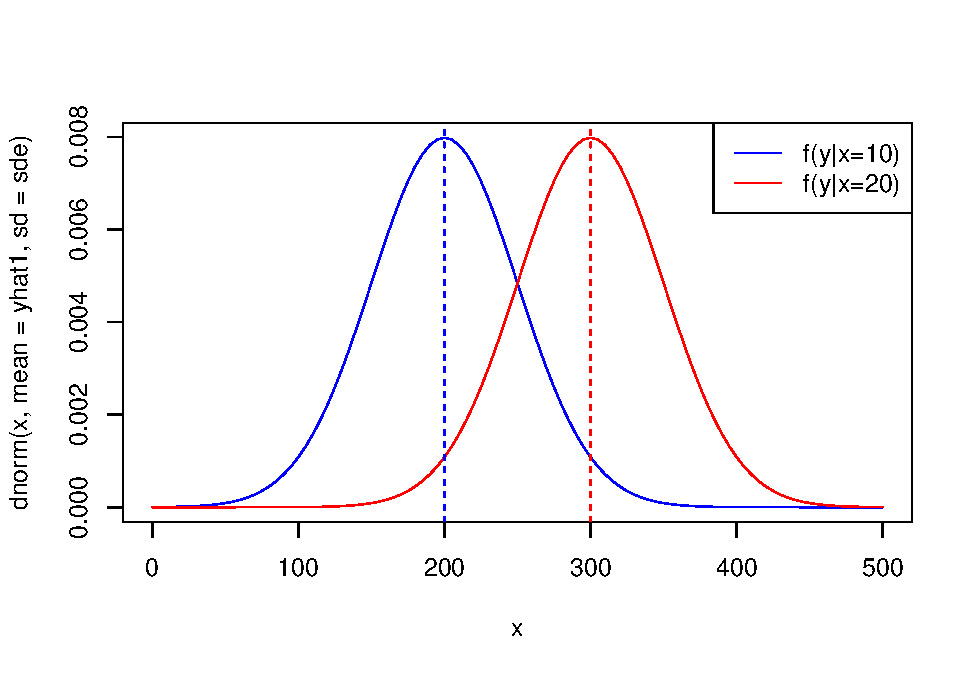
\includegraphics{Econometrics_files/figure-latex/unnamed-chunk-26-1.pdf}

Next, we calculate the variance of \(b_2\) and plot the corresponding density function.

\[
\begin{align}
var(b_2)={\sigma^2 \over \sum(x_i−\bar{x})}
\end{align}
\]

\begin{Shaded}
\begin{Highlighting}[]
\NormalTok{x }\OtherTok{\textless{}{-}} \FunctionTok{c}\NormalTok{(}\FunctionTok{rep}\NormalTok{(x1, N}\SpecialCharTok{/}\DecValTok{2}\NormalTok{), }\FunctionTok{rep}\NormalTok{(x2,N}\SpecialCharTok{/}\DecValTok{2}\NormalTok{))}
\NormalTok{xbar }\OtherTok{\textless{}{-}} \FunctionTok{mean}\NormalTok{(x)}
\NormalTok{sumx2 }\OtherTok{\textless{}{-}} \FunctionTok{sum}\NormalTok{((x}\SpecialCharTok{{-}}\NormalTok{xbar)}\SpecialCharTok{\^{}}\DecValTok{2}\NormalTok{)}
\NormalTok{varb2 }\OtherTok{\textless{}{-}}\NormalTok{ sig2e}\SpecialCharTok{/}\NormalTok{sumx2}
\NormalTok{sdb2 }\OtherTok{\textless{}{-}} \FunctionTok{sqrt}\NormalTok{(varb2)}
\NormalTok{leftlim }\OtherTok{\textless{}{-}}\NormalTok{ b2}\DecValTok{{-}3}\SpecialCharTok{*}\NormalTok{sdb2}
\NormalTok{rightlim }\OtherTok{\textless{}{-}}\NormalTok{ b2}\SpecialCharTok{+}\DecValTok{3}\SpecialCharTok{*}\NormalTok{sdb2}
\FunctionTok{curve}\NormalTok{(}\FunctionTok{dnorm}\NormalTok{(x, }\AttributeTok{mean=}\NormalTok{b2, }\AttributeTok{sd=}\NormalTok{sdb2), leftlim, rightlim)}
\FunctionTok{abline}\NormalTok{(}\AttributeTok{v=}\NormalTok{b2, }\AttributeTok{lty=}\DecValTok{2}\NormalTok{)}
\end{Highlighting}
\end{Shaded}

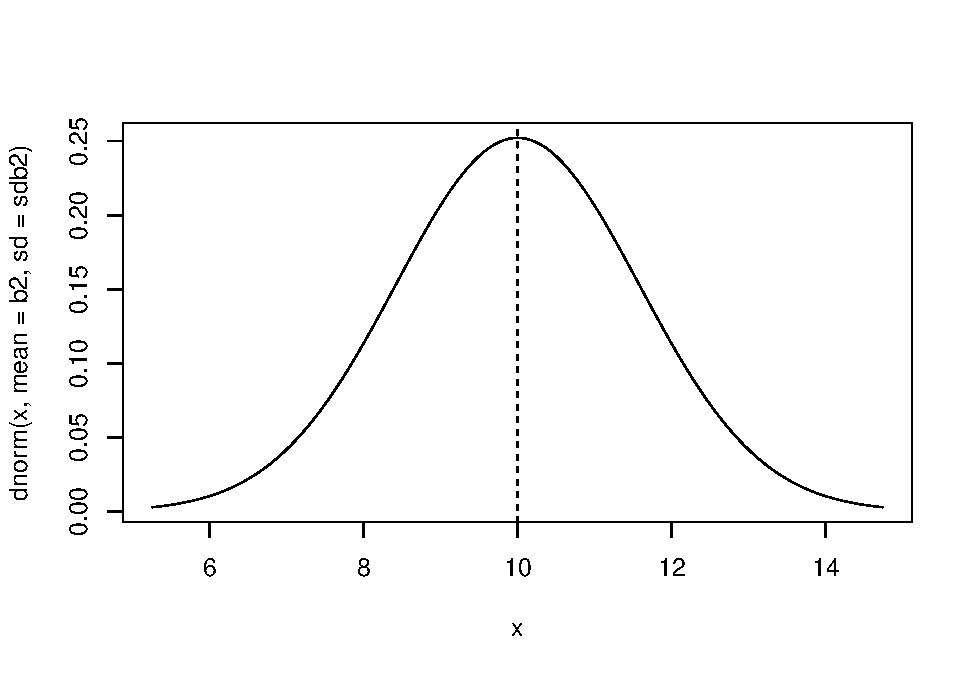
\includegraphics{Econometrics_files/figure-latex/unnamed-chunk-27-1.pdf}

Now, with the same values of \(b_1\) , \(b_2\) , and error standard deviation, we can generate a set of values for \(Y\) , regress \(Y\) on \(X\) , and calculate an estimated values for the coefficient \(b_2\) and its standard error.

\begin{Shaded}
\begin{Highlighting}[]
\FunctionTok{set.seed}\NormalTok{(}\DecValTok{12345}\NormalTok{)}
\NormalTok{y }\OtherTok{\textless{}{-}}\NormalTok{ b1}\SpecialCharTok{+}\NormalTok{b2}\SpecialCharTok{*}\NormalTok{x}\SpecialCharTok{+}\FunctionTok{rnorm}\NormalTok{(N, }\AttributeTok{mean=}\DecValTok{0}\NormalTok{, }\AttributeTok{sd=}\NormalTok{sde)}
\NormalTok{mod6 }\OtherTok{\textless{}{-}} \FunctionTok{lm}\NormalTok{(y}\SpecialCharTok{\textasciitilde{}}\NormalTok{x)}
\NormalTok{b1hat }\OtherTok{\textless{}{-}} \FunctionTok{coef}\NormalTok{(mod6)[[}\DecValTok{1}\NormalTok{]]}
\NormalTok{b2hat }\OtherTok{\textless{}{-}} \FunctionTok{coef}\NormalTok{(mod6)[[}\DecValTok{2}\NormalTok{]]}
\NormalTok{mod6summary }\OtherTok{\textless{}{-}} \FunctionTok{summary}\NormalTok{(mod6) }\CommentTok{\#the summary contains the standard errors}
\NormalTok{seb2hat }\OtherTok{\textless{}{-}} \FunctionTok{coef}\NormalTok{(mod6summary)[}\DecValTok{2}\NormalTok{,}\DecValTok{2}\NormalTok{]}
\end{Highlighting}
\end{Shaded}

The results are \(b_2=11.64\) and \(s_e(b_2)=1.64\). The strength of a Monte Carlo simulation is, however, the possibility of repeating the estimation of the regression parameters for a large number of automatically generated samples. Thus, we can obtain a large number of values for a parameter, say \(b_2\) , and then determine its sampling characteristics. For instance, if the mean of these values is close to the initially asumed value \(b_2= 10\), we conclude that our estimator (the method of estimating the parameter) is unbiased.

We are going to use this time the values of \(X\) in the food dataset, and generate \(Y\) using the linear model with \(b_1=100\) and \(b_2= 10.\)

\begin{Shaded}
\begin{Highlighting}[]
\FunctionTok{data}\NormalTok{(}\StringTok{"food"}\NormalTok{)}
\NormalTok{N }\OtherTok{\textless{}{-}} \DecValTok{40}
\NormalTok{sde }\OtherTok{\textless{}{-}} \DecValTok{50}
\NormalTok{x }\OtherTok{\textless{}{-}}\NormalTok{ food}\SpecialCharTok{$}\NormalTok{income}
\NormalTok{nrsim }\OtherTok{\textless{}{-}} \DecValTok{1000}
\NormalTok{b1 }\OtherTok{\textless{}{-}} \DecValTok{100}
\NormalTok{b2 }\OtherTok{\textless{}{-}} \DecValTok{10}
\NormalTok{vb2 }\OtherTok{\textless{}{-}} \FunctionTok{numeric}\NormalTok{(nrsim) }\CommentTok{\#stores the estimates of b2}
\ControlFlowTok{for}\NormalTok{ (i }\ControlFlowTok{in} \DecValTok{1}\SpecialCharTok{:}\NormalTok{nrsim)\{}
  \FunctionTok{set.seed}\NormalTok{(}\DecValTok{12345}\SpecialCharTok{+}\DecValTok{10}\SpecialCharTok{*}\NormalTok{i)}
\NormalTok{  y }\OtherTok{\textless{}{-}}\NormalTok{ b1}\SpecialCharTok{+}\NormalTok{b2}\SpecialCharTok{*}\NormalTok{x}\SpecialCharTok{+}\FunctionTok{rnorm}\NormalTok{(N, }\AttributeTok{mean=}\DecValTok{0}\NormalTok{, }\AttributeTok{sd=}\NormalTok{sde)}
\NormalTok{  mod7 }\OtherTok{\textless{}{-}} \FunctionTok{lm}\NormalTok{(y}\SpecialCharTok{\textasciitilde{}}\NormalTok{x)}
\NormalTok{  vb2[i] }\OtherTok{\textless{}{-}} \FunctionTok{coef}\NormalTok{(mod7)[[}\DecValTok{2}\NormalTok{]]}
\NormalTok{\}}
\NormalTok{mb2 }\OtherTok{\textless{}{-}} \FunctionTok{mean}\NormalTok{(vb2)}
\NormalTok{seb2 }\OtherTok{\textless{}{-}} \FunctionTok{sd}\NormalTok{(vb2)}
\end{Highlighting}
\end{Shaded}

The mean and standard deviation of the estimated 40 values of \(b_2\) are, respectively, 9.974985 and 1.152632. Figure bellow shows the simulated distribution of \(b_2\) and the theoretical one.

\begin{Shaded}
\begin{Highlighting}[]
\FunctionTok{plot}\NormalTok{(}\FunctionTok{density}\NormalTok{(vb2))}
\FunctionTok{curve}\NormalTok{(}\FunctionTok{dnorm}\NormalTok{(x, mb2, seb2), }\AttributeTok{col=}\StringTok{"red"}\NormalTok{, }\AttributeTok{add=}\ConstantTok{TRUE}\NormalTok{)}
\FunctionTok{legend}\NormalTok{(}\StringTok{"topright"}\NormalTok{, }\AttributeTok{legend=}\FunctionTok{c}\NormalTok{(}\StringTok{"true"}\NormalTok{, }\StringTok{"simulated"}\NormalTok{), }
       \AttributeTok{lty=}\DecValTok{1}\NormalTok{, }\AttributeTok{col=}\FunctionTok{c}\NormalTok{(}\StringTok{"red"}\NormalTok{, }\StringTok{"black"}\NormalTok{))}
\end{Highlighting}
\end{Shaded}

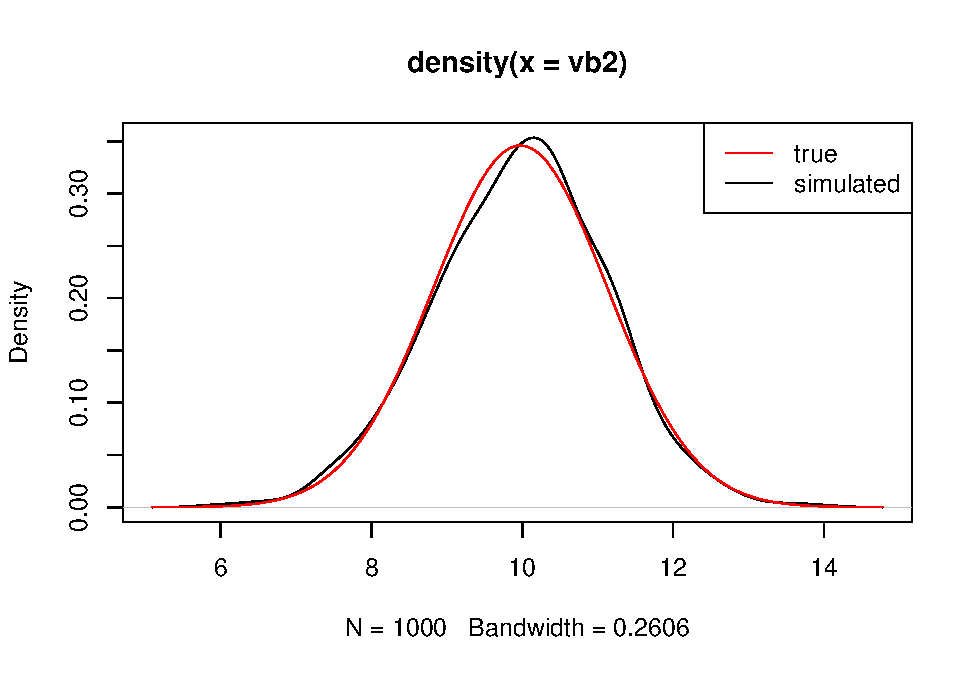
\includegraphics{Econometrics_files/figure-latex/unnamed-chunk-30-1.pdf}

\begin{Shaded}
\begin{Highlighting}[]
\FunctionTok{hist}\NormalTok{(vb2, }\AttributeTok{prob=}\ConstantTok{TRUE}\NormalTok{, }\AttributeTok{ylim=}\FunctionTok{c}\NormalTok{(}\DecValTok{0}\NormalTok{,.}\DecValTok{4}\NormalTok{))}
\FunctionTok{curve}\NormalTok{(}\FunctionTok{dnorm}\NormalTok{(x, }\AttributeTok{mean=}\NormalTok{mb2, }\AttributeTok{sd=}\NormalTok{seb2), }\AttributeTok{col=}\StringTok{"red"}\NormalTok{, }\AttributeTok{add=}\ConstantTok{TRUE}\NormalTok{)}
\end{Highlighting}
\end{Shaded}

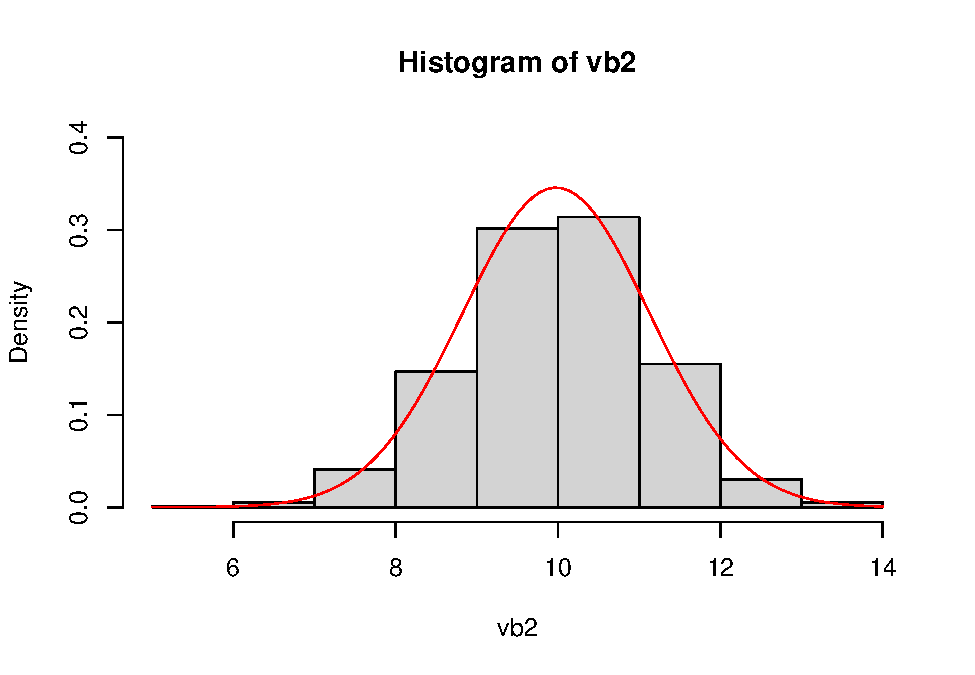
\includegraphics{Econometrics_files/figure-latex/unnamed-chunk-30-2.pdf}

\begin{Shaded}
\begin{Highlighting}[]
\FunctionTok{rm}\NormalTok{(}\AttributeTok{list=}\FunctionTok{ls}\NormalTok{()) }\CommentTok{\# Caution: this clears the Environment}
\end{Highlighting}
\end{Shaded}

\hypertarget{referensi}{%
\chapter{Referensi}\label{referensi}}

  \bibliography{book.bib,packages.bib}

\end{document}
